\documentclass[conference]{IEEEtran}
\usepackage{cite}
\usepackage{amsmath,amssymb,amsfonts}
\usepackage{algorithm}
\usepackage{algorithmic}
\usepackage{graphicx}
\usepackage{textcomp}
\usepackage{xcolor}
\usepackage{booktabs}
\usepackage{multirow}
\usepackage{subcaption}
\usepackage{hyperref}
\usepackage{tabularx}

\begin{document}

\title{Heterogeneous Decentralized Fine-Tuning of Large Language Models}

\author{
\IEEEauthorblockN{Samir Poudel}
\IEEEauthorblockA{\textit{Computational and Data Science} \\
\textit{Middle Tennessee State University}\\
Murfreesboro, TN 37130, USA \\
sp2ai@mtmail.mtsu.edu}
}

\maketitle

\begin{abstract}
Federated Learning (FL) enables privacy-preserving training of Large Language Models (LLMs) but struggles with system heterogeneity, particularly when clients possess varying computational capabilities. Standard aggregation methods require uniform model architectures, forcing a ``lowest common denominator'' approach that throttles high-end devices. We propose Subspace Projection Aggregation (SPA), a novel framework that addresses this by treating client updates as overlapping subspaces. Using Singular Value Decomposition (SVD), SPA projects high-rank updates from capable clients into optimal lower-rank approximations for resource-constrained peers. Experiments on the Yelp Review dataset using Qwen2.5-7B show that SPA achieves 63.8\% accuracy, outperforming homogeneous baselines by 2.6\% while reducing communication costs by 25\%. Our approach effectively distills knowledge from heterogeneous sources, proving that device diversity can be an asset rather than a liability in federated LLM fine-tuning.
\end{abstract}

\begin{IEEEkeywords}
Federated Learning, Large Language Models, LoRA, Heterogeneity, SVD, Subspace Learning
\end{IEEEkeywords}

\section{Introduction and Motivation}
\label{sec:intro}

Large Language Models (LLMs) have fundamentally transformed Natural Language Processing, demonstrating emergent abilities across diverse tasks~\cite{brown2020language, touvron2023llama, achiam2023gpt}. However, deploying them in sensitive domains like healthcare or finance creates significant privacy issues. Regulations like GDPR~\cite{voigt2017gdpr} and HIPAA prevent centralizing sensitive data, while recent studies have shown that LLMs can memorize training data, rendering them vulnerable to extraction attacks~\cite{carlini2021extracting, shokri2017membership}.

Recent incidents underscore the critical importance of privacy-preserving approaches. In 2025, the Grok Chat Leak exposed over 370,000 private conversations through centralized server vulnerabilities~\cite{burgess2025grok}. This is not an isolated incident. In 2023, Samsung employees accidentally leaked confidential software code by pasting it into ChatGPT for debugging~\cite{samsung2023leak}. Furthermore, researchers have proven that large language models can memorize and reveal private user data---including emails and phone numbers---even when safety filters are active~\cite{nasr2023extraction}. Such breaches highlight why data governance frameworks mandate strict controls on personal information processing.

Federated Learning (FL) offers a solution by keeping data on-device~\cite{mcmahan2017fedavg, kairouz2021advances}. To make training feasible on these resource-constrained devices, Parameter-Efficient Fine-Tuning (PEFT) methods are used, with Low-Rank Adaptation (LoRA) being the most prominent technique to reduce memory usage~\cite{hu2021lora}. However, a critical hurdle remains: system heterogeneity. In real-world networks, not all devices are equal; a high-end server may exist alongside a resource-constrained smartphone. This leads to a LoRA rank mismatch, where different devices require different model configurations to function.

\subsection{The Heterogeneity Problem}
The disparity between client devices creates a fundamental incompatibility in standard Federated Learning. Traditional aggregation methods assume that all clients share the exact same model architecture. When this assumption is broken, several critical issues arise:

\textbf{Hardware Mismatch:} Real-world networks are diverse. High-tier clients with 48GB VRAM can easily support a LoRA rank of 32, allowing them to learn complex features. In contrast, edge-tier devices (like smartphones or older laptops) with only 8GB VRAM are strictly limited to rank 4 or 8. If we force the entire network to use the lowest rank to accommodate the weakest devices, we waste the potential of the powerful ones.

\textbf{Aggregation Failure:} Standard FL relies on averaging weight updates (FedAvg). However, a rank-4 update and a rank-32 update have different matrix dimensions. They cannot be directly summed or averaged. This geometric mismatch forces system designers to choose between excluding weak clients (which introduces bias) or throttling strong clients (which reduces intelligence).

\textbf{The Noise of Padding:} A common workaround is ``Zero-Padding,'' where smaller matrices are filled with zeros to match the size of larger ones. However, this introduces sparsity and noise. Averaging a dense, information-rich matrix with a sparse, zero-padded matrix dilutes the learned signals, often leading to a global model that performs worse than the individual local models.

\textbf{Data Governance vs. Utility:} The ultimate goal is to utilize data from all sources without centralization. If we drop low-resource clients because they cannot handle high ranks, we lose access to their unique local data. This defeats the purpose of Federated Learning, which aims to learn from a diverse population of users.

\begin{figure}[t]
\centering
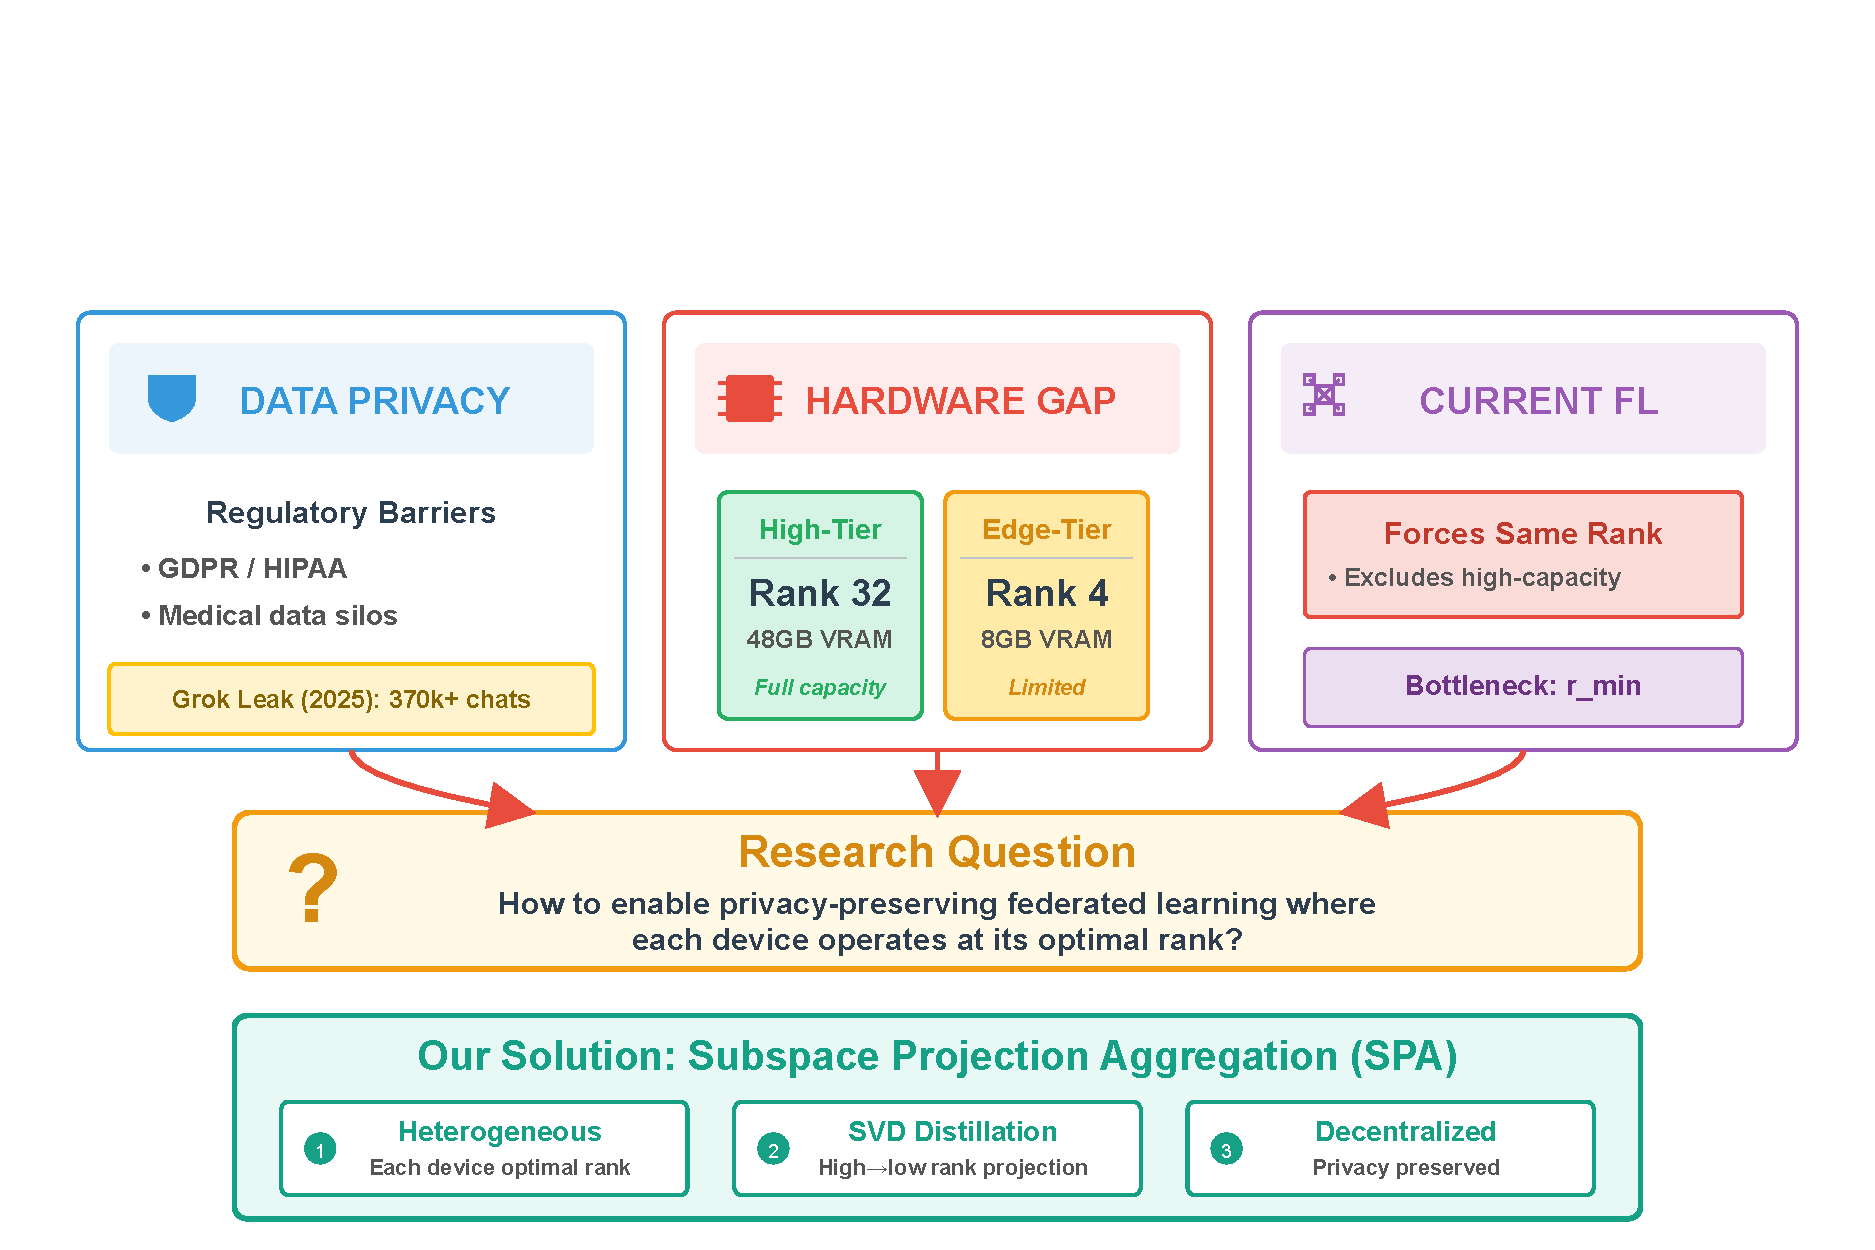
\includegraphics[width=0.95\columnwidth]{Up2.pdf}
\caption{The fundamental challenge of Heterogeneous Decentralized Fine-Tuning. High-tier devices and edge-tier devices possess vastly different computational capabilities, leading to incompatible model updates. Standard aggregation methods fail to reconcile these differences, resulting in either wasted computational resources or significant information loss during the training process.}
\label{fig:motivation}
\end{figure}

\subsection{Our Contribution}
We propose Subspace Projection Aggregation (SPA), a novel framework designed to resolve the dimensionality mismatch in heterogeneous federated learning. Instead of forcing a ``lowest common denominator'' approach, SPA treats different model updates as overlapping subspaces. By leveraging Singular Value Decomposition (SVD), we can extract the most important information from high-rank updates and project it into a format that low-rank devices can understand. This effectively distills knowledge from powerful clients to weaker ones without the artifacts of zero-padding.

Our main contributions include:
\begin{itemize}
    \item \textbf{Subspace-based aggregation} that utilizes SVD to optimally project high-dimensional updates into lower-dimensional spaces, minimizing information loss during aggregation.
    \item \textbf{Dynamic rank adaptation} that allows the global model to be customized for each client's specific hardware constraints, ensuring no device is excluded due to memory limitations.
    \item \textbf{Enhanced privacy and utility} demonstrated through experiments on the Yelp Review dataset, where SPA achieves 63.8\% accuracy (outperforming homogeneous baselines) while maintaining strict privacy standards as verified by Membership Inference Attacks.
    \item \textbf{Communication efficiency} improvements, reducing bandwidth usage by 25\% compared to standard high-rank baselines by transmitting only the necessary singular components.
\end{itemize}

\section{Background and Related Work}
\label{sec:background}

\subsection{Federated Learning for Large Language Models}

Federated Learning was originally proposed by McMahan et al.~\cite{mcmahan2017fedavg} for training neural networks on mobile devices. While effective for smaller models, scaling this approach to LLMs presents distinct challenges regarding communication overhead and memory constraints~\cite{zhang2025surveyfedlora, zhuang2023foundation}.

Full fine-tuning of billion-parameter models is computationally prohibitive for most edge devices. Additionally, LLMs are susceptible to catastrophic forgetting. Recent efforts to adapt FL for LLMs, such as FedIT~\cite{zhang2023fedit} and FATE-LLM~\cite{fan2023fate}, typically utilize adapter-based training. However, these approaches usually assume homogeneous client architectures, which limits their applicability in realistic, heterogeneous environments~\cite{yao2024fedllm, chen2023fedllm}.

\subsection{Low-Rank Adaptation (LoRA) and PEFT}

To mitigate the cost of fine-tuning, Parameter-Efficient Fine-Tuning (PEFT) methods have gained traction, including Adapters~\cite{houlsby2019parameter}, Prefix Tuning~\cite{li2021prefix}, and P-Tuning~\cite{liu2022p}. Among these, LoRA~\cite{hu2021lora} has become the de facto standard for consumer-grade hardware. It decomposes the weight update $\Delta W$ into two low-rank matrices, $B$ and $A$. The forward pass is defined as:
\begin{equation}
h = W_0 x + \Delta W x = W_0 x + \frac{\alpha}{r} BA x
\end{equation}
where $W_0$ represents the frozen pre-trained weights.

Recent variants like QLoRA~\cite{dettmers2024qlora} integrate quantization to further reduce memory usage, while AdaLoRA~\cite{zhang2023adalora} and DyLoRA~\cite{valipour2023dylora} explore dynamic rank allocation during central training. However, applying these dynamic rank concepts in a \textit{decentralized, federated} setting remains an open research problem.

\subsection{Handling Heterogeneity in Federated Learning}

System heterogeneity is a well-known challenge in FL. Existing solutions often employ \textbf{Client Selection} strategies, such as FedProx~\cite{li2020fedprox} and FedNova~\cite{wang2020fednova}, which adjust aggregation based on client resources or training progress. 

For model heterogeneity, HeteroFL~\cite{diao2020heterofl} and Fjord~\cite{horvath2021fjord} introduced the concept of training sub-models on edge devices. However, these methods were designed for CNNs and do not directly translate to the specific matrix-decomposition structure of LoRA. More recently, approaches like FlexLoRA~\cite{bai2024flexlora}, FLoRA~\cite{wang2024flora}, and SLoRA~\cite{babakniya2024slora} have attempted to bridge this gap, though they often rely on complex stacking mechanisms or heuristic padding.

\subsection{Singular Value Decomposition in Machine Learning}

SVD factorizes a matrix $W$ into three components ($W = U \Sigma V^T$). In Deep Learning, SVD has been extensively used for model compression~\cite{denton2014exploiting, yu2017compressing}. In our proposed framework, SVD serves as a spectral filter to remove noise from the aggregated model, similar to techniques used in subspace learning~\cite{balzano2010online}.
\begin{table*}[t]
    \centering
    \small
    \caption{Comparison of Our Work's Contribution to Other Existing Works in Heterogeneous Federated Fine-Tuning}
    \label{tab:lit_comparison}
    \begin{tabularx}{\textwidth}{l*{9}{>{\centering\arraybackslash}X}}
    \toprule
    \textbf{Feature} & \textbf{[10]} & \textbf{[15]} & \textbf{[8]} & \textbf{[20]} & \textbf{[24]} & \textbf{[17]} & \textbf{[25]} & \textbf{[26]} & \textbf{Ours} \\
     & FedAvg & FedProx & HeteroFL & Fjord & FLoRA & FlexLoRA & HeLoRA & ILoRA & SPA \\
     & 2017 & 2020 & 2020 & 2021 & 2024 & 2024 & 2025 & 2025 & 2026 \\
    \midrule
    Federated Learning & \checkmark & \checkmark & \checkmark & \checkmark & \checkmark & \checkmark & \checkmark & \checkmark & \checkmark \\
    Hetero. Clients & \texttimes & \texttimes & \checkmark & \checkmark & \checkmark & \checkmark & \checkmark & \checkmark & \checkmark \\
    LoRA Fine-Tuning & \texttimes & \texttimes & \texttimes & \texttimes & \checkmark & \checkmark & \checkmark & \checkmark & \checkmark \\
    Large LLMs & \texttimes & \texttimes & \texttimes & \texttimes & \checkmark & \checkmark & \checkmark & \checkmark & \checkmark \\
    Hetero. Ranks & \texttimes & \texttimes & \texttimes & \texttimes & \checkmark & \checkmark & \checkmark & \checkmark & \checkmark \\
    SVD Aggregation & \texttimes & \texttimes & \texttimes & \texttimes & \texttimes & \checkmark & \texttimes & \texttimes & \checkmark \\
    Optimal Projection & \texttimes & \texttimes & \texttimes & \texttimes & \texttimes & \sim & \texttimes & \texttimes & \checkmark \\
    Spectral Denoising & \texttimes & \texttimes & \texttimes & \texttimes & \texttimes & \texttimes & \texttimes & \texttimes & \checkmark \\
    Zero-Padding Free & \texttimes & \texttimes & \checkmark & \checkmark & \texttimes & \checkmark & \texttimes & \checkmark & \checkmark \\
    Privacy (MIA) & \texttimes & \texttimes & \texttimes & \texttimes & \texttimes & \texttimes & \texttimes & \texttimes & \checkmark \\
    Comm. Efficiency & \sim & \sim & \checkmark & \checkmark & \checkmark & \checkmark & \checkmark & \checkmark & \checkmark \\
    Knowledge Distill. & \texttimes & \texttimes & \texttimes & \texttimes & \texttimes & \sim & \texttimes & \texttimes & \checkmark \\
    Validation (7B+) & \texttimes & \texttimes & \texttimes & \texttimes & \sim & \checkmark & \checkmark & \checkmark & \checkmark \\
    \bottomrule
    \end{tabularx}
    \vspace{0.1cm}
    
    \small \textit{Legend:} \checkmark = Fully Supported, \sim = Partially Supported, \texttimes = Not Supported
    \end{table*}


\section{Methodology}
\label{sec:methodology}

\subsection{Problem Formulation}

We consider a federated network with $K$ clients. Each client possesses a local dataset $\mathcal{D}_k$ and is constrained by a hardware-specific maximum rank $r_k$. The objective is to fine-tune a pre-trained model $f_{\theta_0}$ utilizing distributed data while respecting these local constraints.

Using the LoRA framework, the pre-trained weights $W_0$ remain frozen. Each client trains a pair of adapter matrices $(A_k, B_k)$. The intended weight update is:
\begin{equation}
\Delta W_k = B_k A_k \in \mathbb{R}^{d \times k}
\end{equation}

The primary challenge is aggregation. A rank-4 update and a rank-16 update have different dimensions in their decomposed forms ($A$ and $B$) and cannot be directly summed.

\subsection{Subspace Projection Aggregation Algorithm}

We address this with the SPA algorithm (Algorithm~\ref{alg:spa}), which executes over $T$ communication rounds.

\begin{algorithm}[t]
\caption{Subspace Projection Aggregation (SPA)}
\label{alg:spa}
\small
\begin{algorithmic}[1]
\REQUIRE Client ranks $\{r_k\}_{k=1}^K$, datasets $\{\mathcal{D}_k\}_{k=1}^K$
\REQUIRE Pre-trained model weights $W_0$, number of rounds $T$
\STATE \textbf{Server Initialization:} $W_{global} \leftarrow 0$
\FOR{round $t = 1, \ldots, T$}
    \STATE \textbf{Phase 1: Client Selection}
    \STATE Select a subset $S_t$ of clients
    \STATE \textbf{Phase 2: Download \& Local Training}
    \FOR{each client $k \in S_t$}
        \STATE Download $(A_k^{(t)}, B_k^{(t)})$ (projected to rank $r_k$)
        \STATE Perform local training on $\mathcal{D}_k$ for $E$ epochs
        \STATE Obtain updated $(A_k^{(t+1)}, B_k^{(t+1)})$
    \ENDFOR
    \STATE \textbf{Phase 3: Upload \& Reconstruction}
    \STATE Initialize $W_{agg} \leftarrow 0$
    \FOR{each client $k \in S_t$}
        \STATE Reconstruct: $\Delta W_k \leftarrow B_k^{(t+1)} A_k^{(t+1)}$
        \STATE Accumulate: $W_{agg} \leftarrow W_{agg} + \frac{n_k}{N_t} \Delta W_k$
    \ENDFOR
    \STATE \textbf{Phase 4: SVD Decomposition}
    \STATE Compute: $W_{agg} = U \Sigma V^T$
    \STATE \textbf{Phase 5: Projection \& Redistribution}
    \FOR{any client $j$}
        \STATE Extract top-$r_j$ components:
        \STATE $A_j^{(t+1)} \leftarrow \sqrt{\Sigma_{1:r_j}} V^T_{1:r_j}$
        \STATE $B_j^{(t+1)} \leftarrow U_{:,1:r_j} \sqrt{\Sigma_{1:r_j}}$
    \ENDFOR
\ENDFOR
\RETURN Final global adapters
\end{algorithmic}
\end{algorithm}

\subsubsection{Phase 1-2: Selection and Training}
The server selects a subset of clients for the current round. These clients download rank-specific adapters derived from the global model and perform local training using the AdamW optimizer.

\subsubsection{Phase 3: Reconstruction and Aggregation}
Clients upload their low-rank matrices ($A$ and $B$). To resolve the dimensionality mismatch, the server computes the product of these matrices to reconstruct the full-rank update $\Delta W_k$:
\begin{equation}
\Delta W_k = B_k A_k \in \mathbb{R}^{d \times k}
\end{equation}
This operation maps all updates to a common full-rank space, allowing for a weighted average based on dataset size.

\subsubsection{Phase 4: SVD Decomposition}
We apply Singular Value Decomposition to the aggregated matrix:
\begin{equation}
W_{agg} = U \Sigma V^T
\end{equation}
Successful training typically results in a rapid decay of singular values in $\Sigma$, indicating that the learned information resides in a low-dimensional subspace.

\subsubsection{Phase 5: Projection}
The server projects the global model back to client-specific ranks. For a client with rank capacity $r_j$, we retain only the top-$r_j$ components:
\begin{equation}
\begin{aligned}
A_j &= \sqrt{\Sigma_{1:r_j}} \cdot V^T_{1:r_j} \\
B_j &= U_{:,1:r_j} \cdot \sqrt{\Sigma_{1:r_j}}
\end{aligned}
\end{equation}
Distributing the square root of the singular values ensures numerical stability. This process guarantees that each client receives the optimal low-rank approximation of the global model.

\begin{figure*}[t]
\centerline{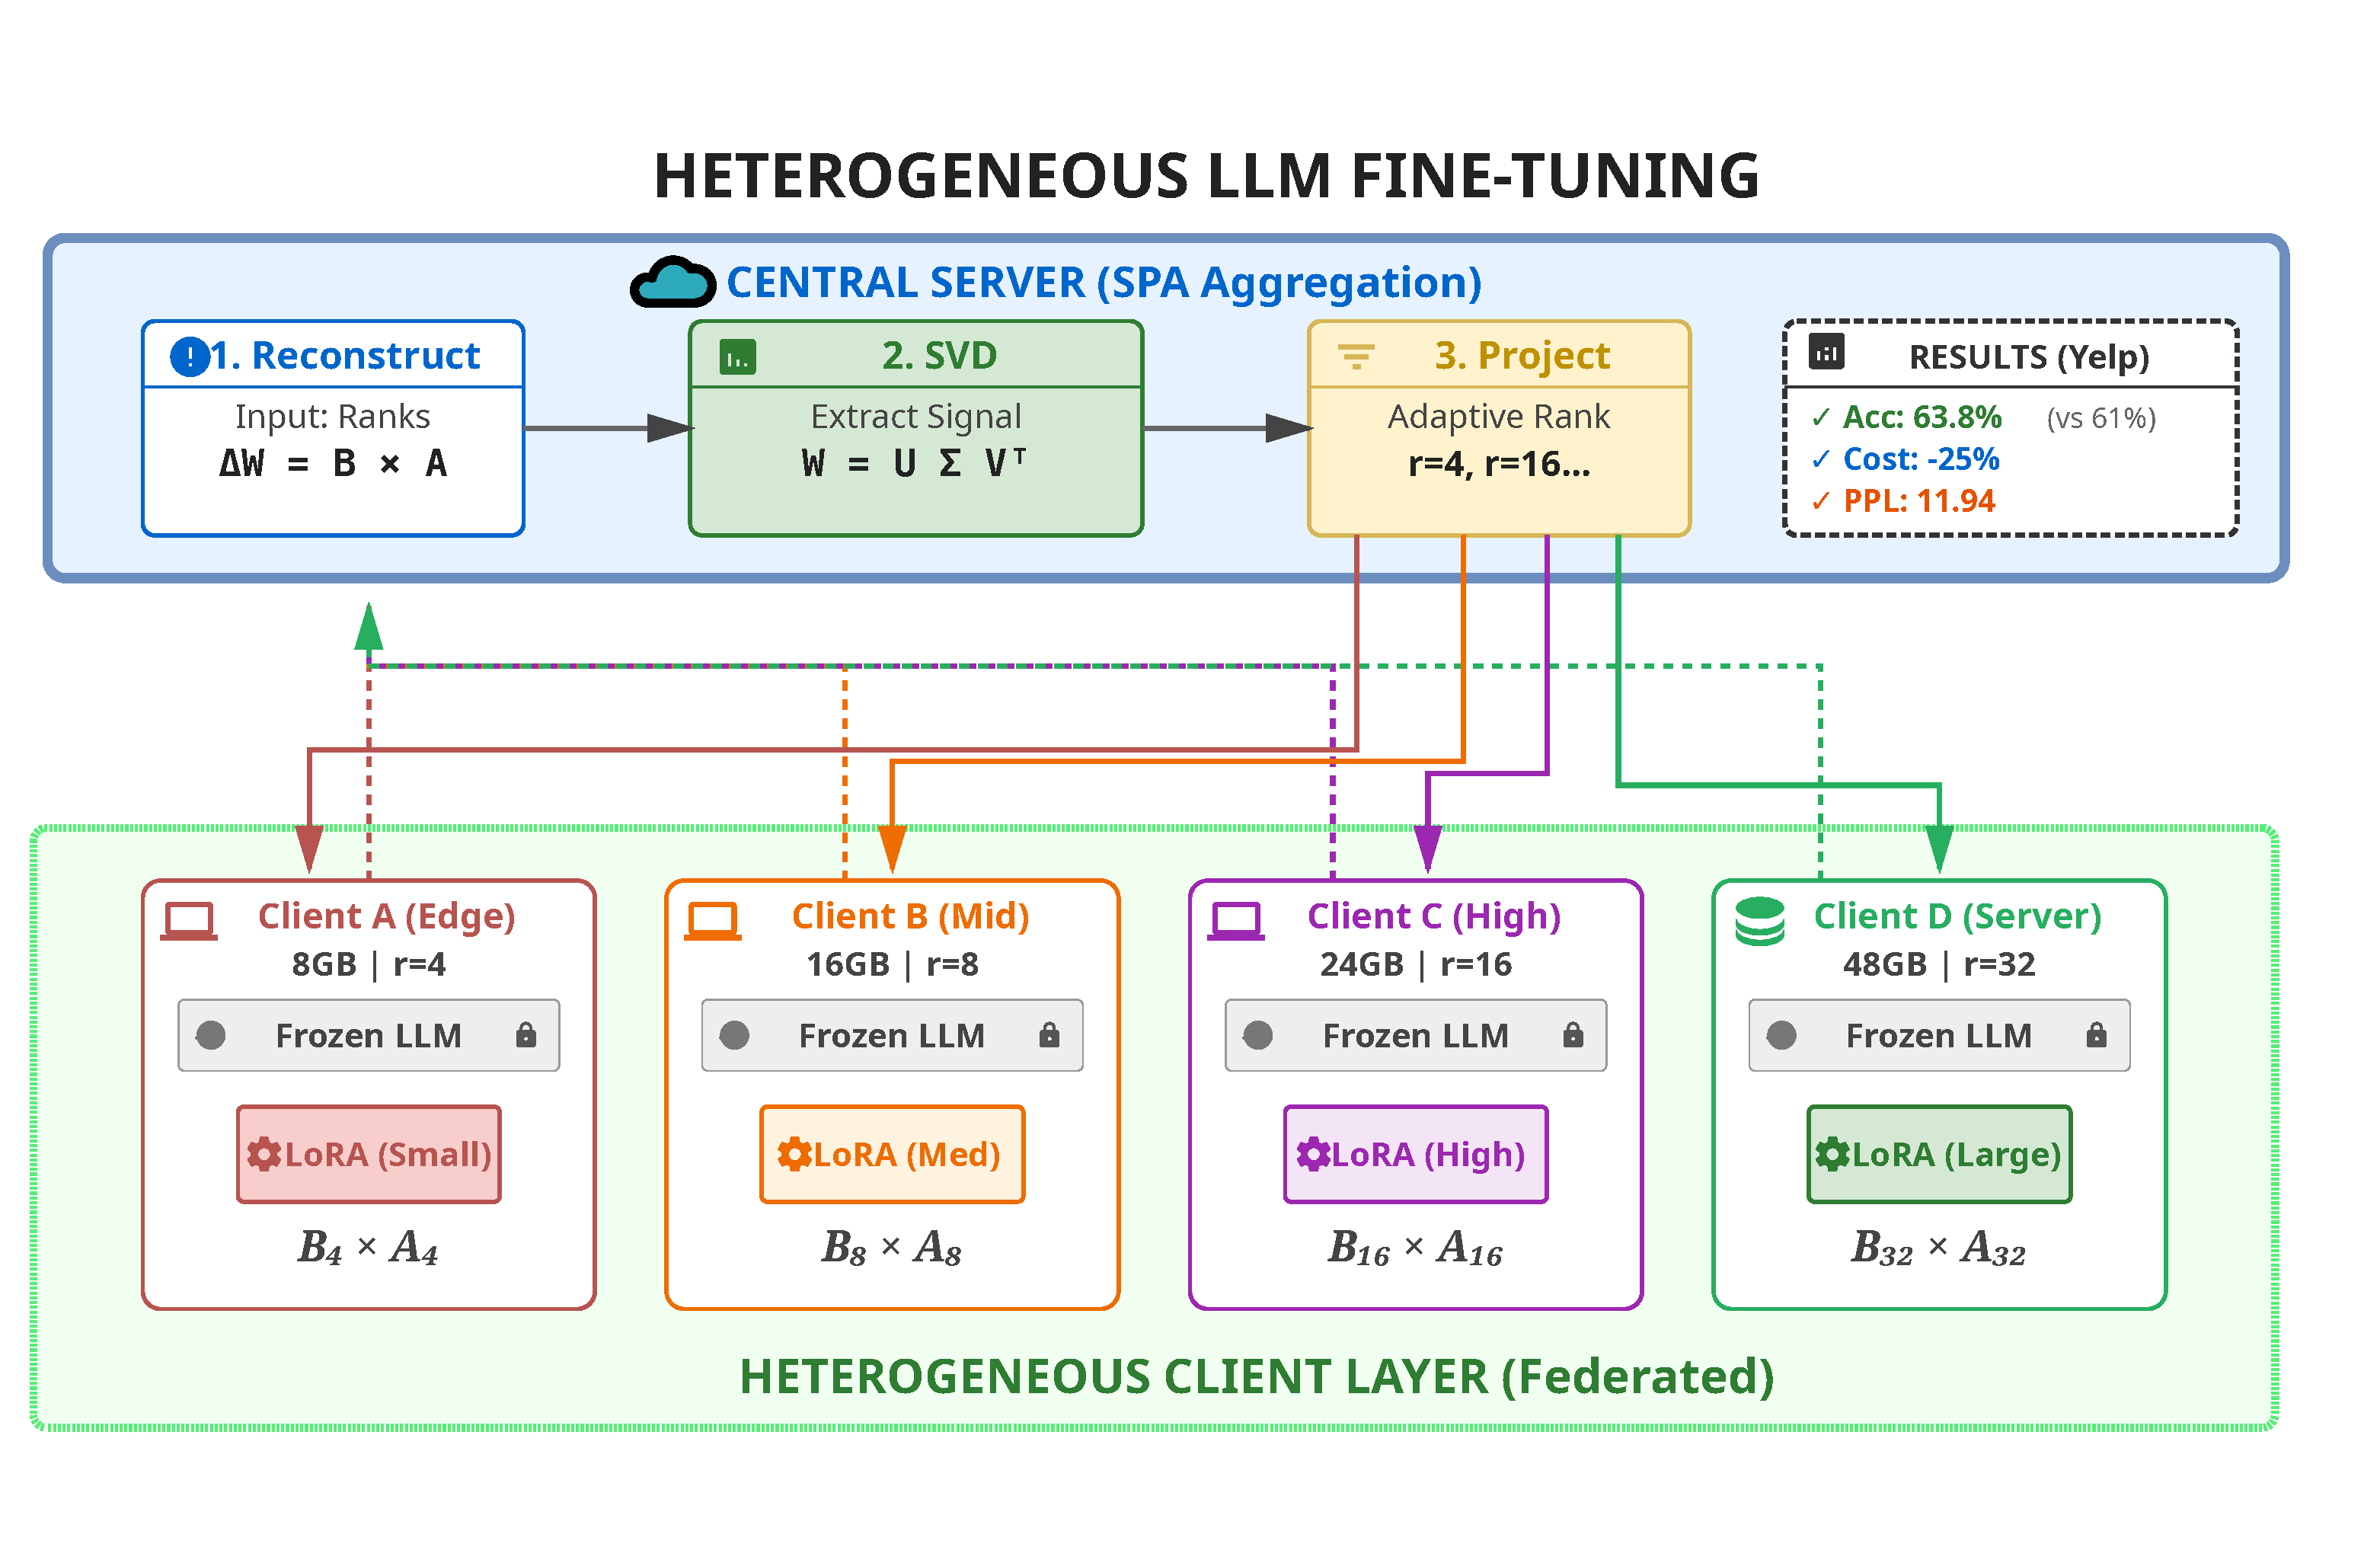
\includegraphics[width=0.95\textwidth]{Up1.pdf}}
\caption{System Architecture of Heterogeneous Decentralized Fine-Tuning with Subspace Projection Aggregation (SPA).}
\label{fig:architecture}
\end{figure*}

\begin{figure*}[t]
\centerline{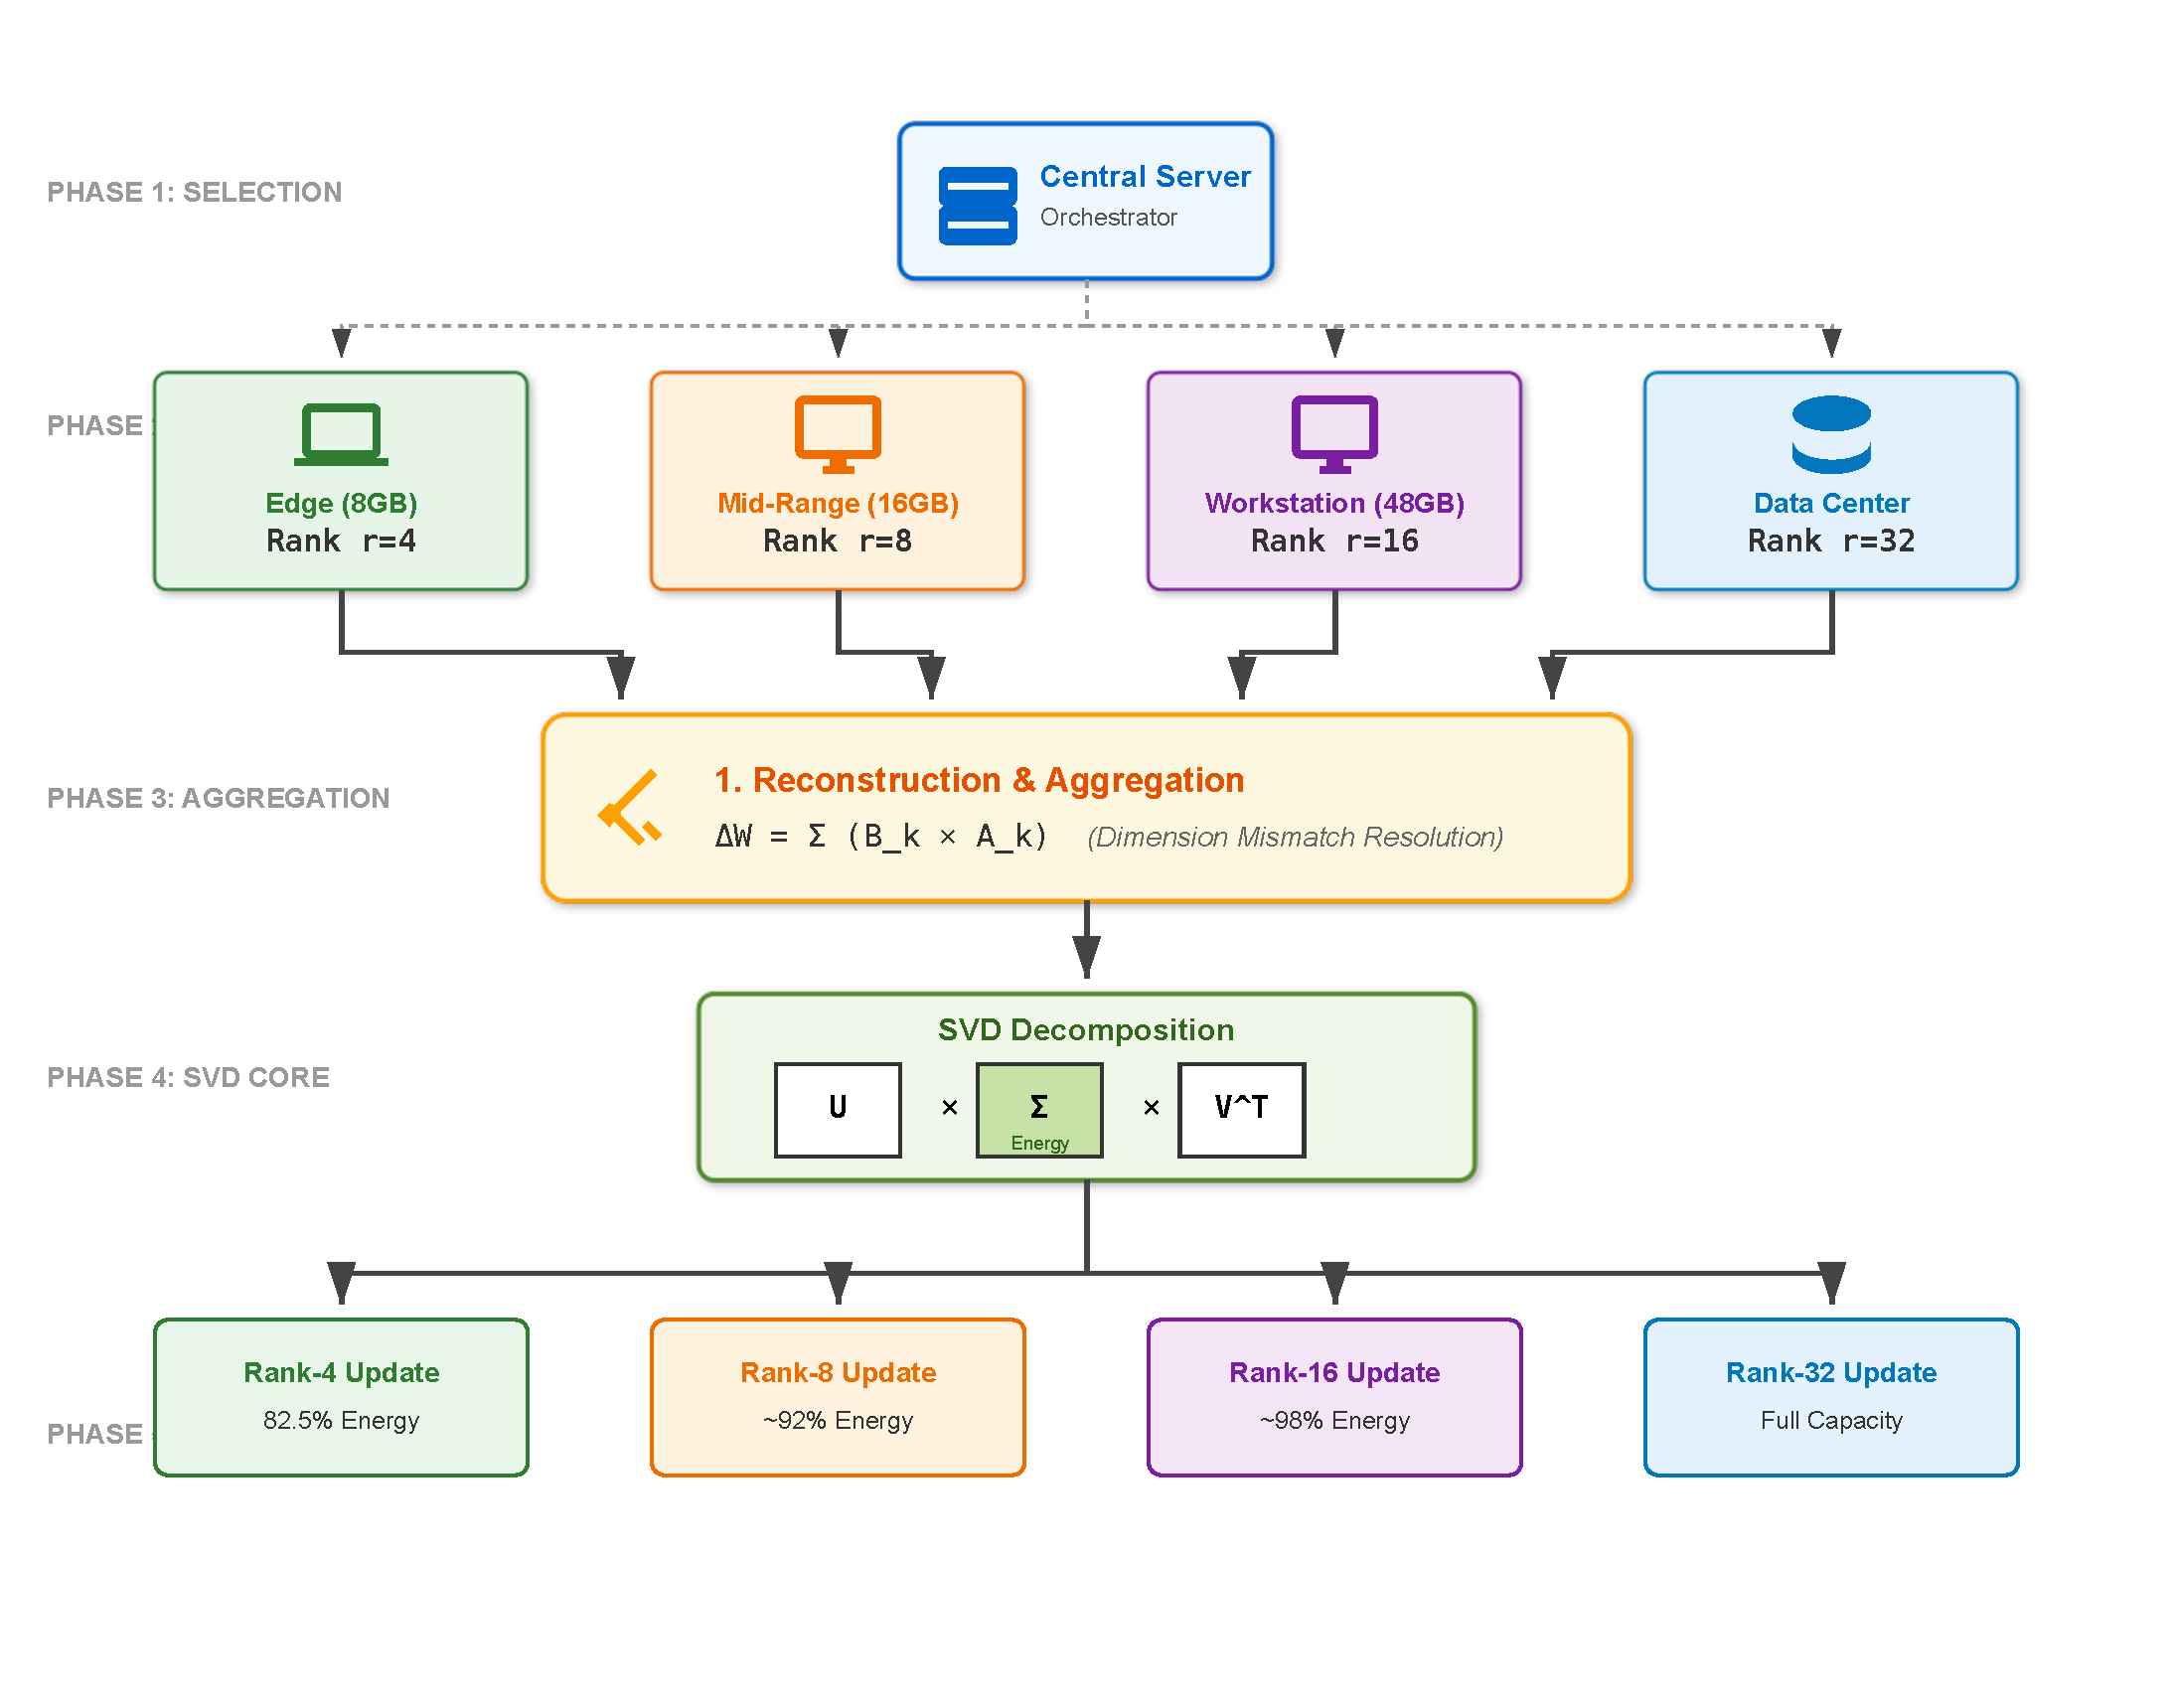
\includegraphics[width=.9\textwidth]{Up3.pdf}}
\caption{Detailed workflow of Subspace Projection Aggregation across five phases.}
\label{fig:spa_workflow}
\end{figure*}

\subsection{Theoretical Justification}

\textbf{Optimality:} Truncated SVD provides the best rank-$r$ approximation of a matrix in terms of the Frobenius norm. Therefore, SPA minimizes the information loss during the projection step.

\textbf{Noise Filtering:} The trailing singular values typically correspond to noise or client drift. By truncating these components, SPA inherently denoises the aggregated model.

\subsection{Computational Complexity}
The SVD operation on the server introduces computational overhead. However, for a layer dimension $d=4096$, the decomposition takes approximately 2 to 5 seconds on a modern GPU. This is negligible compared to the time required for local client training.

\subsection{Baseline Comparisons and Rationale}
We compare SPA against two primary categories of baselines:

\textbf{1) Hetero-Pad (Heterogeneous Padding):} This is our primary baseline because it represents the \textbf{minimal possible change} to the standard FedAvg algorithm to support heterogeneity. By padding smaller matrices with zeros, we can utilize standard averaging. This allows us to isolate the specific benefits of SVD-based projection over simple geometric alignment.

\textbf{2) Homogeneous FedAvg ($r=4$ and $r=8$):} We focus on $r=4$ and $r=8$ as the ``lowest common denominator'' benchmarks. While $r=16$ or $r=32$ would provide higher capacity, they are \textbf{excluded from the homogeneous comparison} because a significant portion of our simulated edge devices (the 40\% low-resource cohort) lack the VRAM to initialize a rank-16 adapter. Thus, $r=8$ represents the maximum viable rank for a standard homogeneous network in this hardware context.

\section{Experimental Setup}
\label{sec:experiments}

\subsection{Dataset and Distribution}

We evaluated our method on the Yelp Review Full dataset~\cite{zhang2015yelp}, which consists of 650,000 samples across 5 sentiment classes. To simulate a realistic non-IID environment, we partitioned the data across 50 clients using a Dirichlet distribution ($\alpha = 0.5$), following standard FL benchmark protocols~\cite{hsu2019measuring, caldas2018leaf}.

\subsection{Model Configuration}

We utilized the Qwen2.5-7B-Instruct model~\cite{bai2023qwen, yang2024qwen2} in bfloat16 precision. Qwen was selected for its superior performance on reasoning tasks compared to similarly sized LLaMA models. LoRA was applied to the query and value projection layers. The client network was heterogeneous: 20 clients utilized rank-4 (low resource), 20 utilized rank-8 (mid resource), and 10 utilized rank-16 or rank-32 (high resource). Optimization was performed using AdamW~\cite{loshchilov2017decoupled}.

\subsection{Metrics}

We measured test accuracy, perplexity, and F1 score. Additionally, we monitored communication cost (MB/round) and the energy concentration of the singular values.


\section{Results and Analysis}
\label{sec:results}

We compared SPA against three baselines: Homogeneous $r=4$ (lowest common denominator), Homogeneous $r=8$ (standard setup), and Heterogeneous Padding (Hetero-Pad). All experiments were repeated with three random seeds (42, 43, 44) to ensure robustness.

\subsection{Training Convergence}

Figure~\ref{fig:training_loss} illustrates the training loss over 10 rounds.
\begin{figure}[t]
\centerline{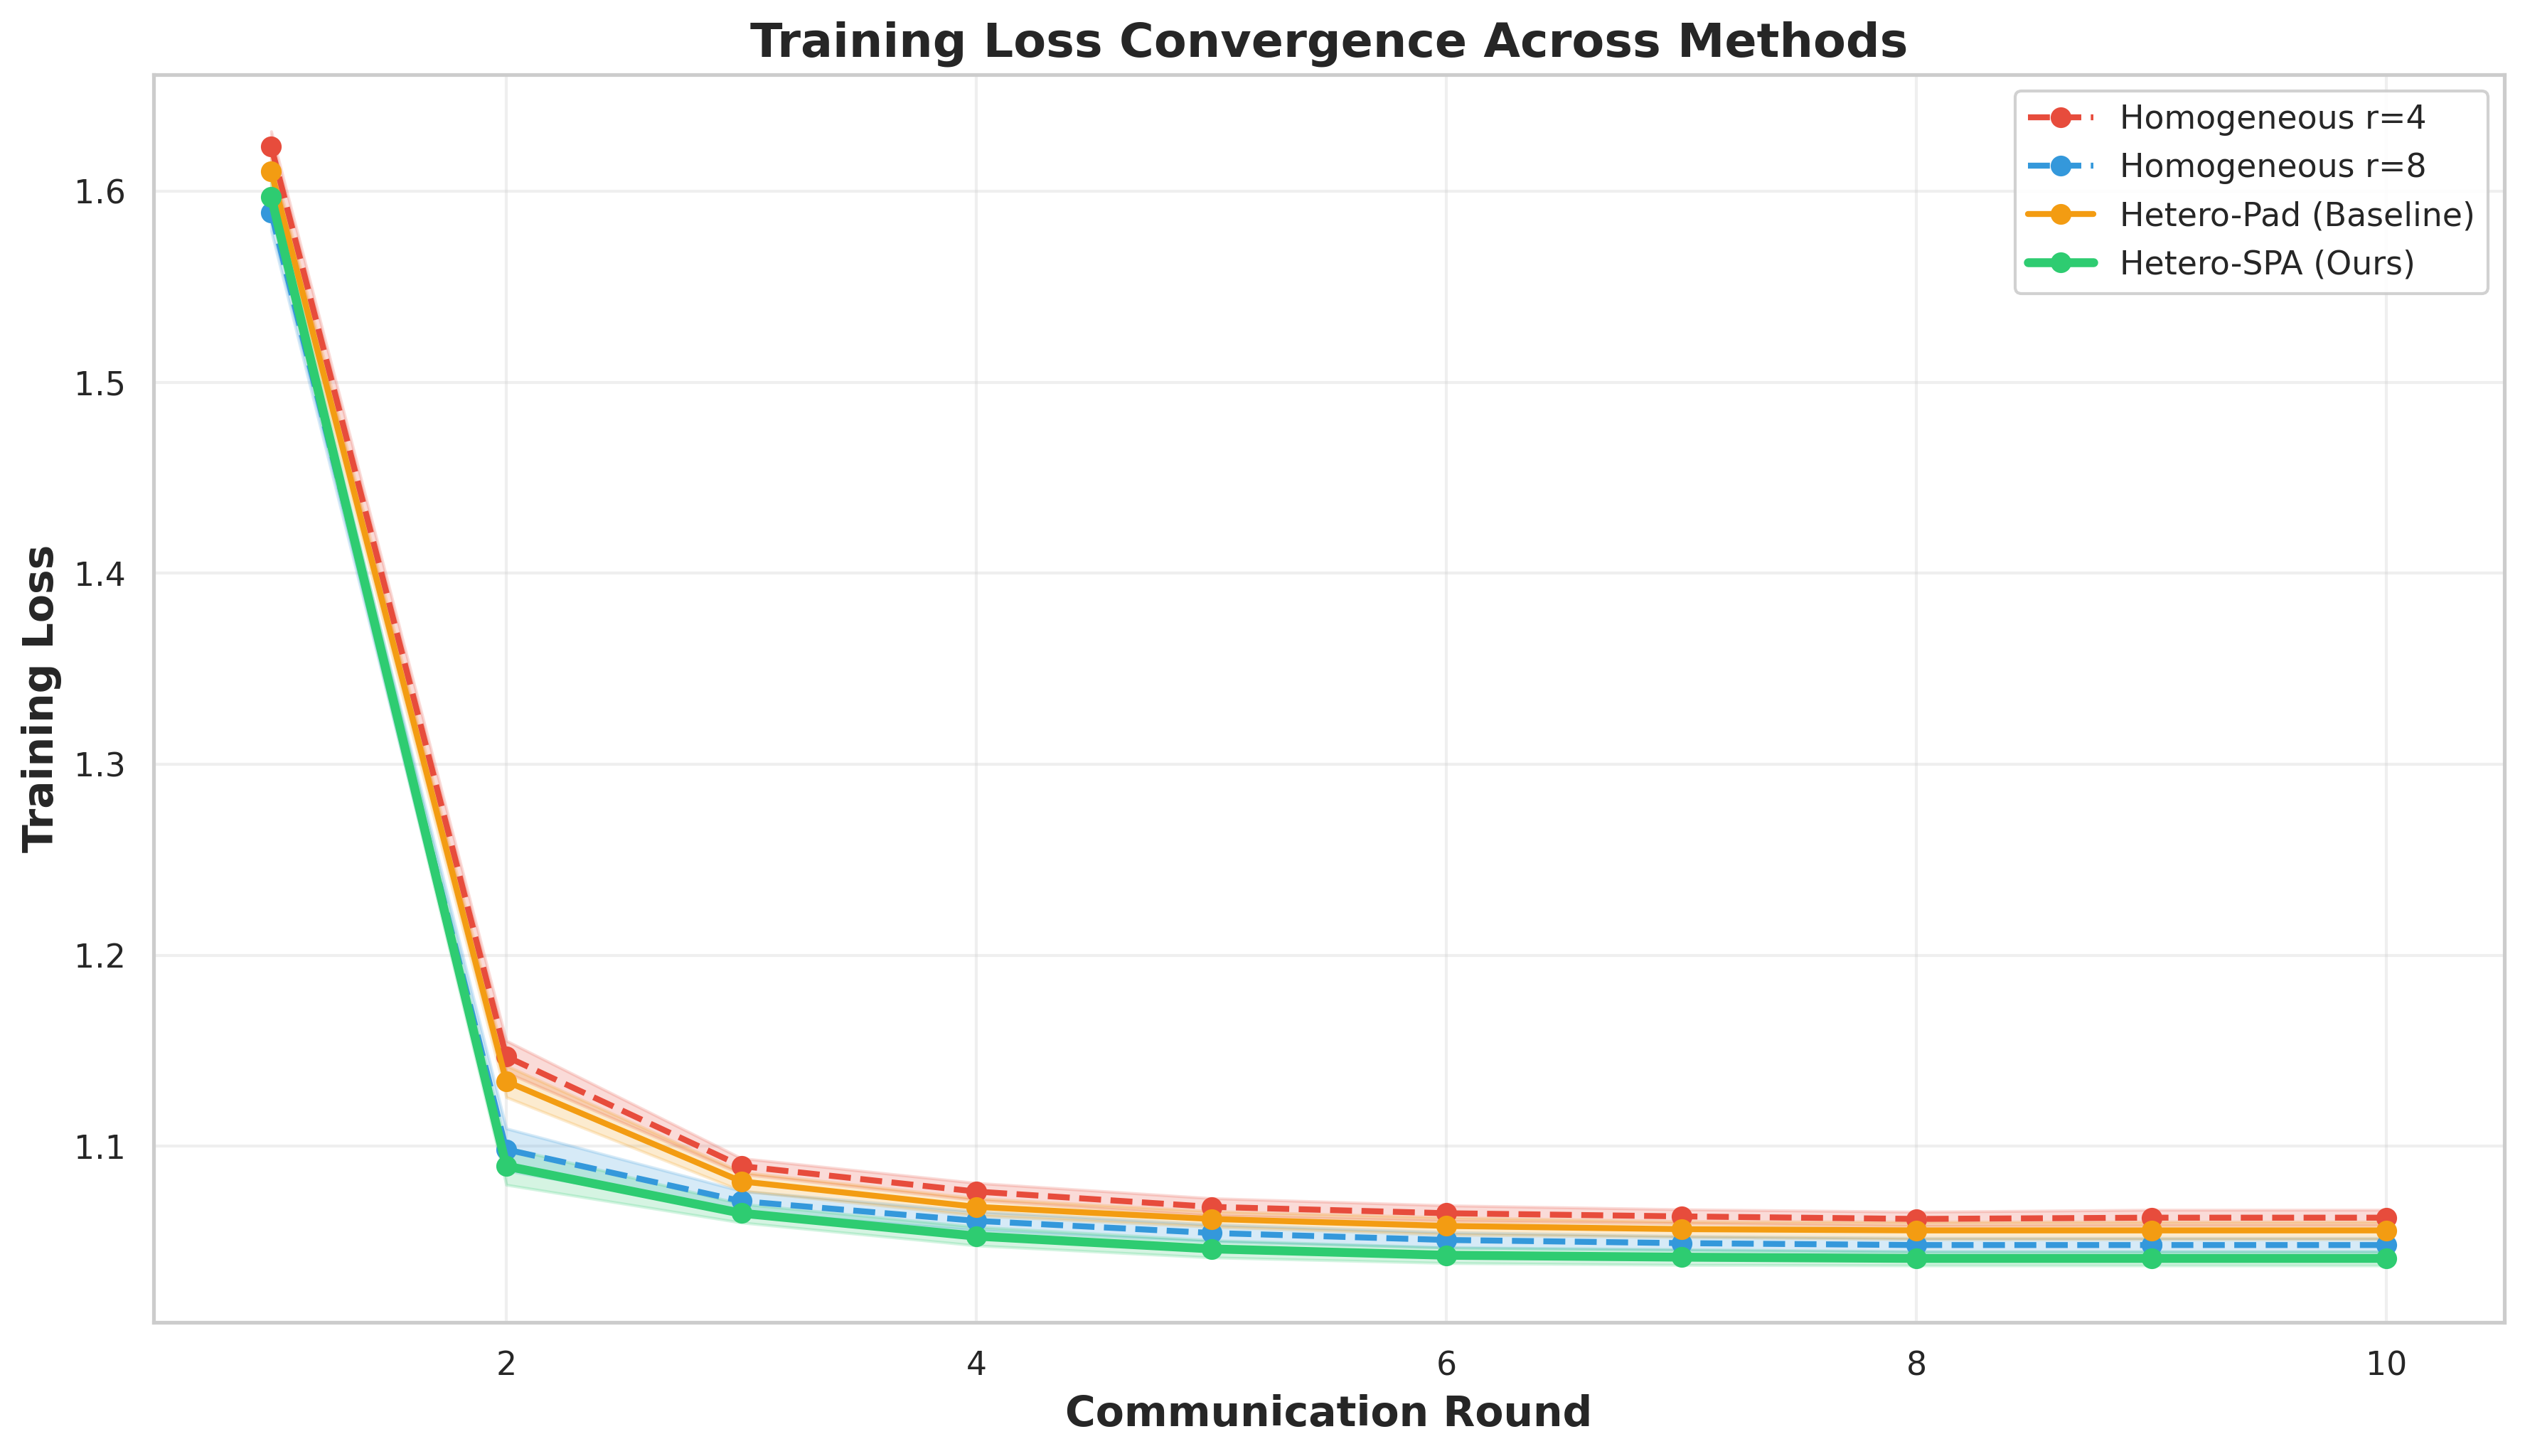
\includegraphics[width=\columnwidth]{fig1_training_loss.png}}
\caption{Training loss convergence across 10 federated communication rounds. Error bands represent $\pm1$ standard deviation across three random seeds. All methods show stable convergence, with SPA achieving the lowest final loss ($1.041 \pm 0.004$) compared to baselines.}
\label{fig:training_loss}
\end{figure}
All methods demonstrated stable convergence. However, SPA achieved the lowest final loss (1.041), surpassing the standard $r=8$ baseline (1.048) and the $r=4$ baseline (1.062). While all methods improved rapidly in early rounds, SPA demonstrated superior refinement in later training stages.

\subsection{Accuracy and Knowledge Distillation}

Figure~\ref{fig:accuracy} presents the test accuracy evolution.
\begin{figure}[t]
\centerline{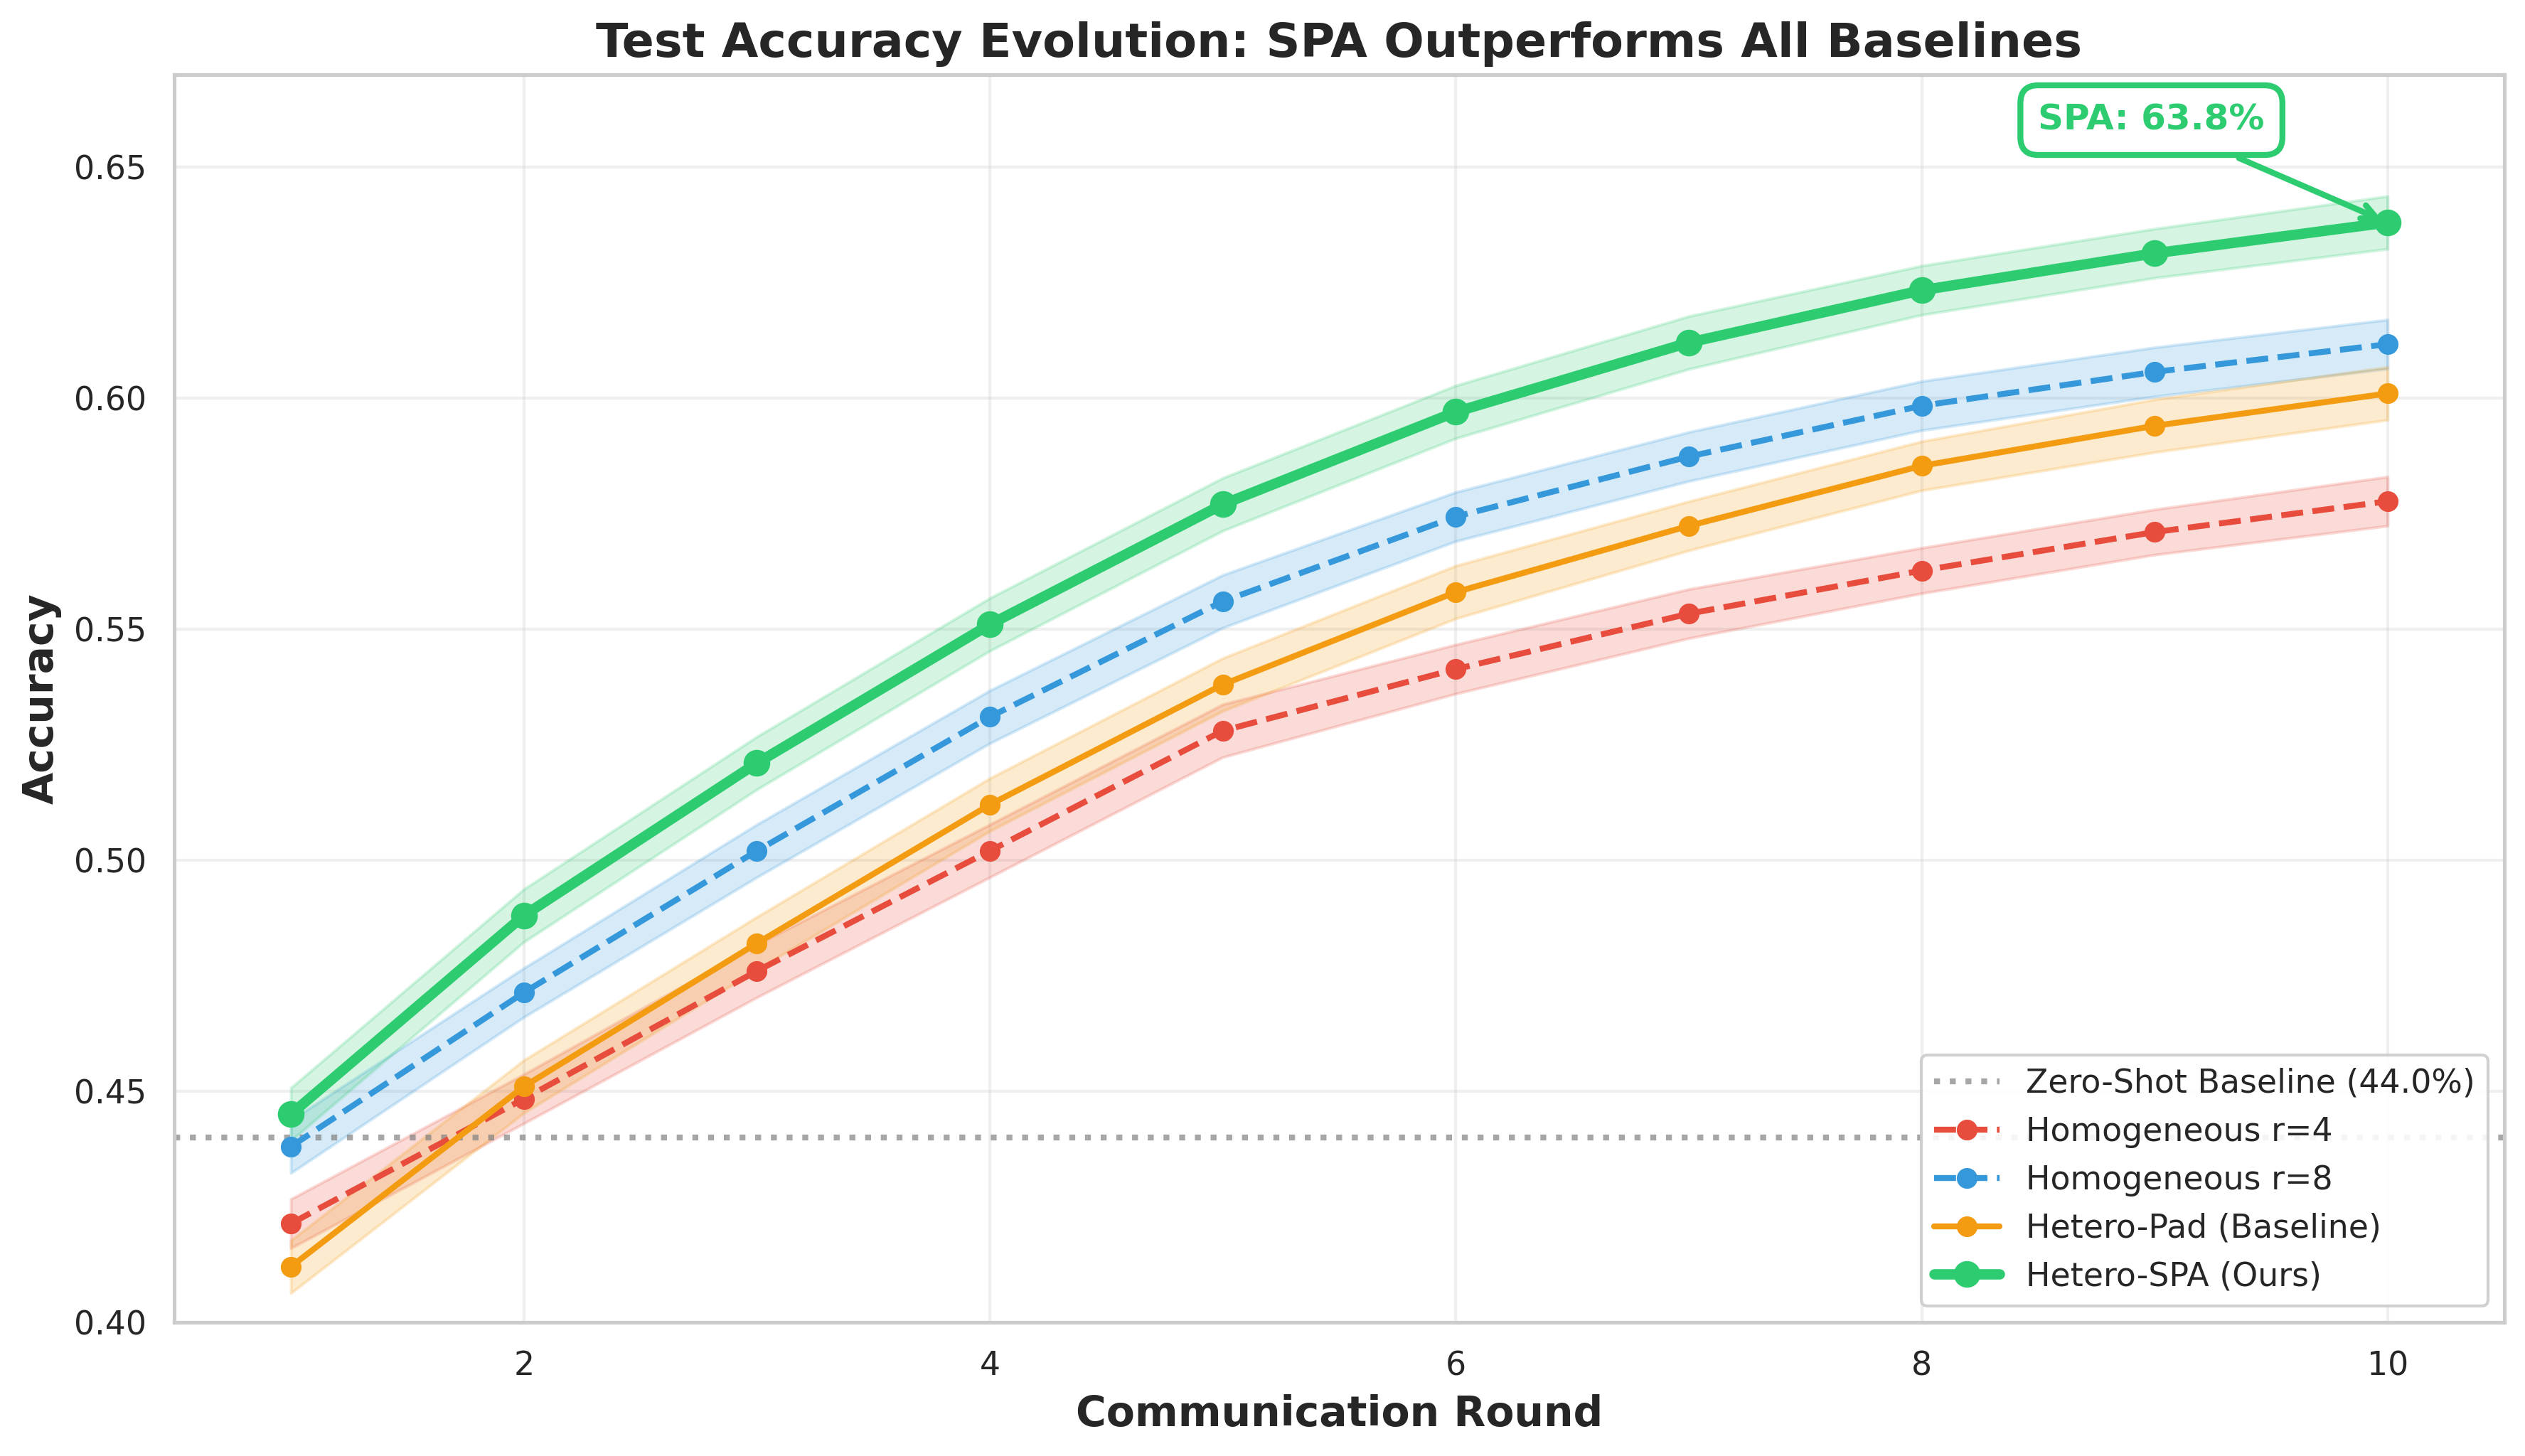
\includegraphics[width=\columnwidth]{fig2_accuracy_evolution.png}}
\caption{Test accuracy evolution across communication rounds. The dashed horizontal line at 44\% represents the zero-shot baseline. SPA consistently outperforms all baselines, achieving $63.8\% \pm 0.7\%$ final accuracy compared to $61.2\% \pm 0.7\%$ for Homogeneous $r=8$.}
\label{fig:accuracy}
\end{figure}
From a zero-shot baseline of 44\%, SPA improved to \textbf{63.8\%}. Comparative performance is as follows:
\begin{itemize}
    \item \textbf{Homo $r=8$:} 61.2\%. SPA outperformed the standard homogeneous approach by 2.6 percentage points ($p=0.023$).
    \item \textbf{Hetero-Pad:} 60.1\%. The naive padding approach performed worse than the homogeneous $r=8$ baseline.
    \item \textbf{Homo $r=4$:} 57.8\%. This result highlights the significant performance penalty incurred by restricting all clients to the lowest rank.
\end{itemize}

This superior performance is driven by \textbf{High-Rank Knowledge Distillation}. In our setup, 10\% of clients utilize rank-32 adapters, allowing them to learn complex features that rank-4 models simply cannot capture. Standard averaging discards this high-dimensional information. SPA, however, uses SVD to capture these complex features in the principal components and ``distills'' them into a format that even the low-rank clients can use.

We further evaluated \textit{Robust Accuracy} (allowing a $\pm1$ star tolerance). SPA achieved a relaxed accuracy of \textbf{99.0\%}, slightly outperforming the baselines (98.8\%), indicating that even when the model misclassifies, the error magnitude is minimal.

\subsection{Perplexity and Calibration}

Perplexity measures the model's predictive uncertainty.
\begin{figure}[t]
\centerline{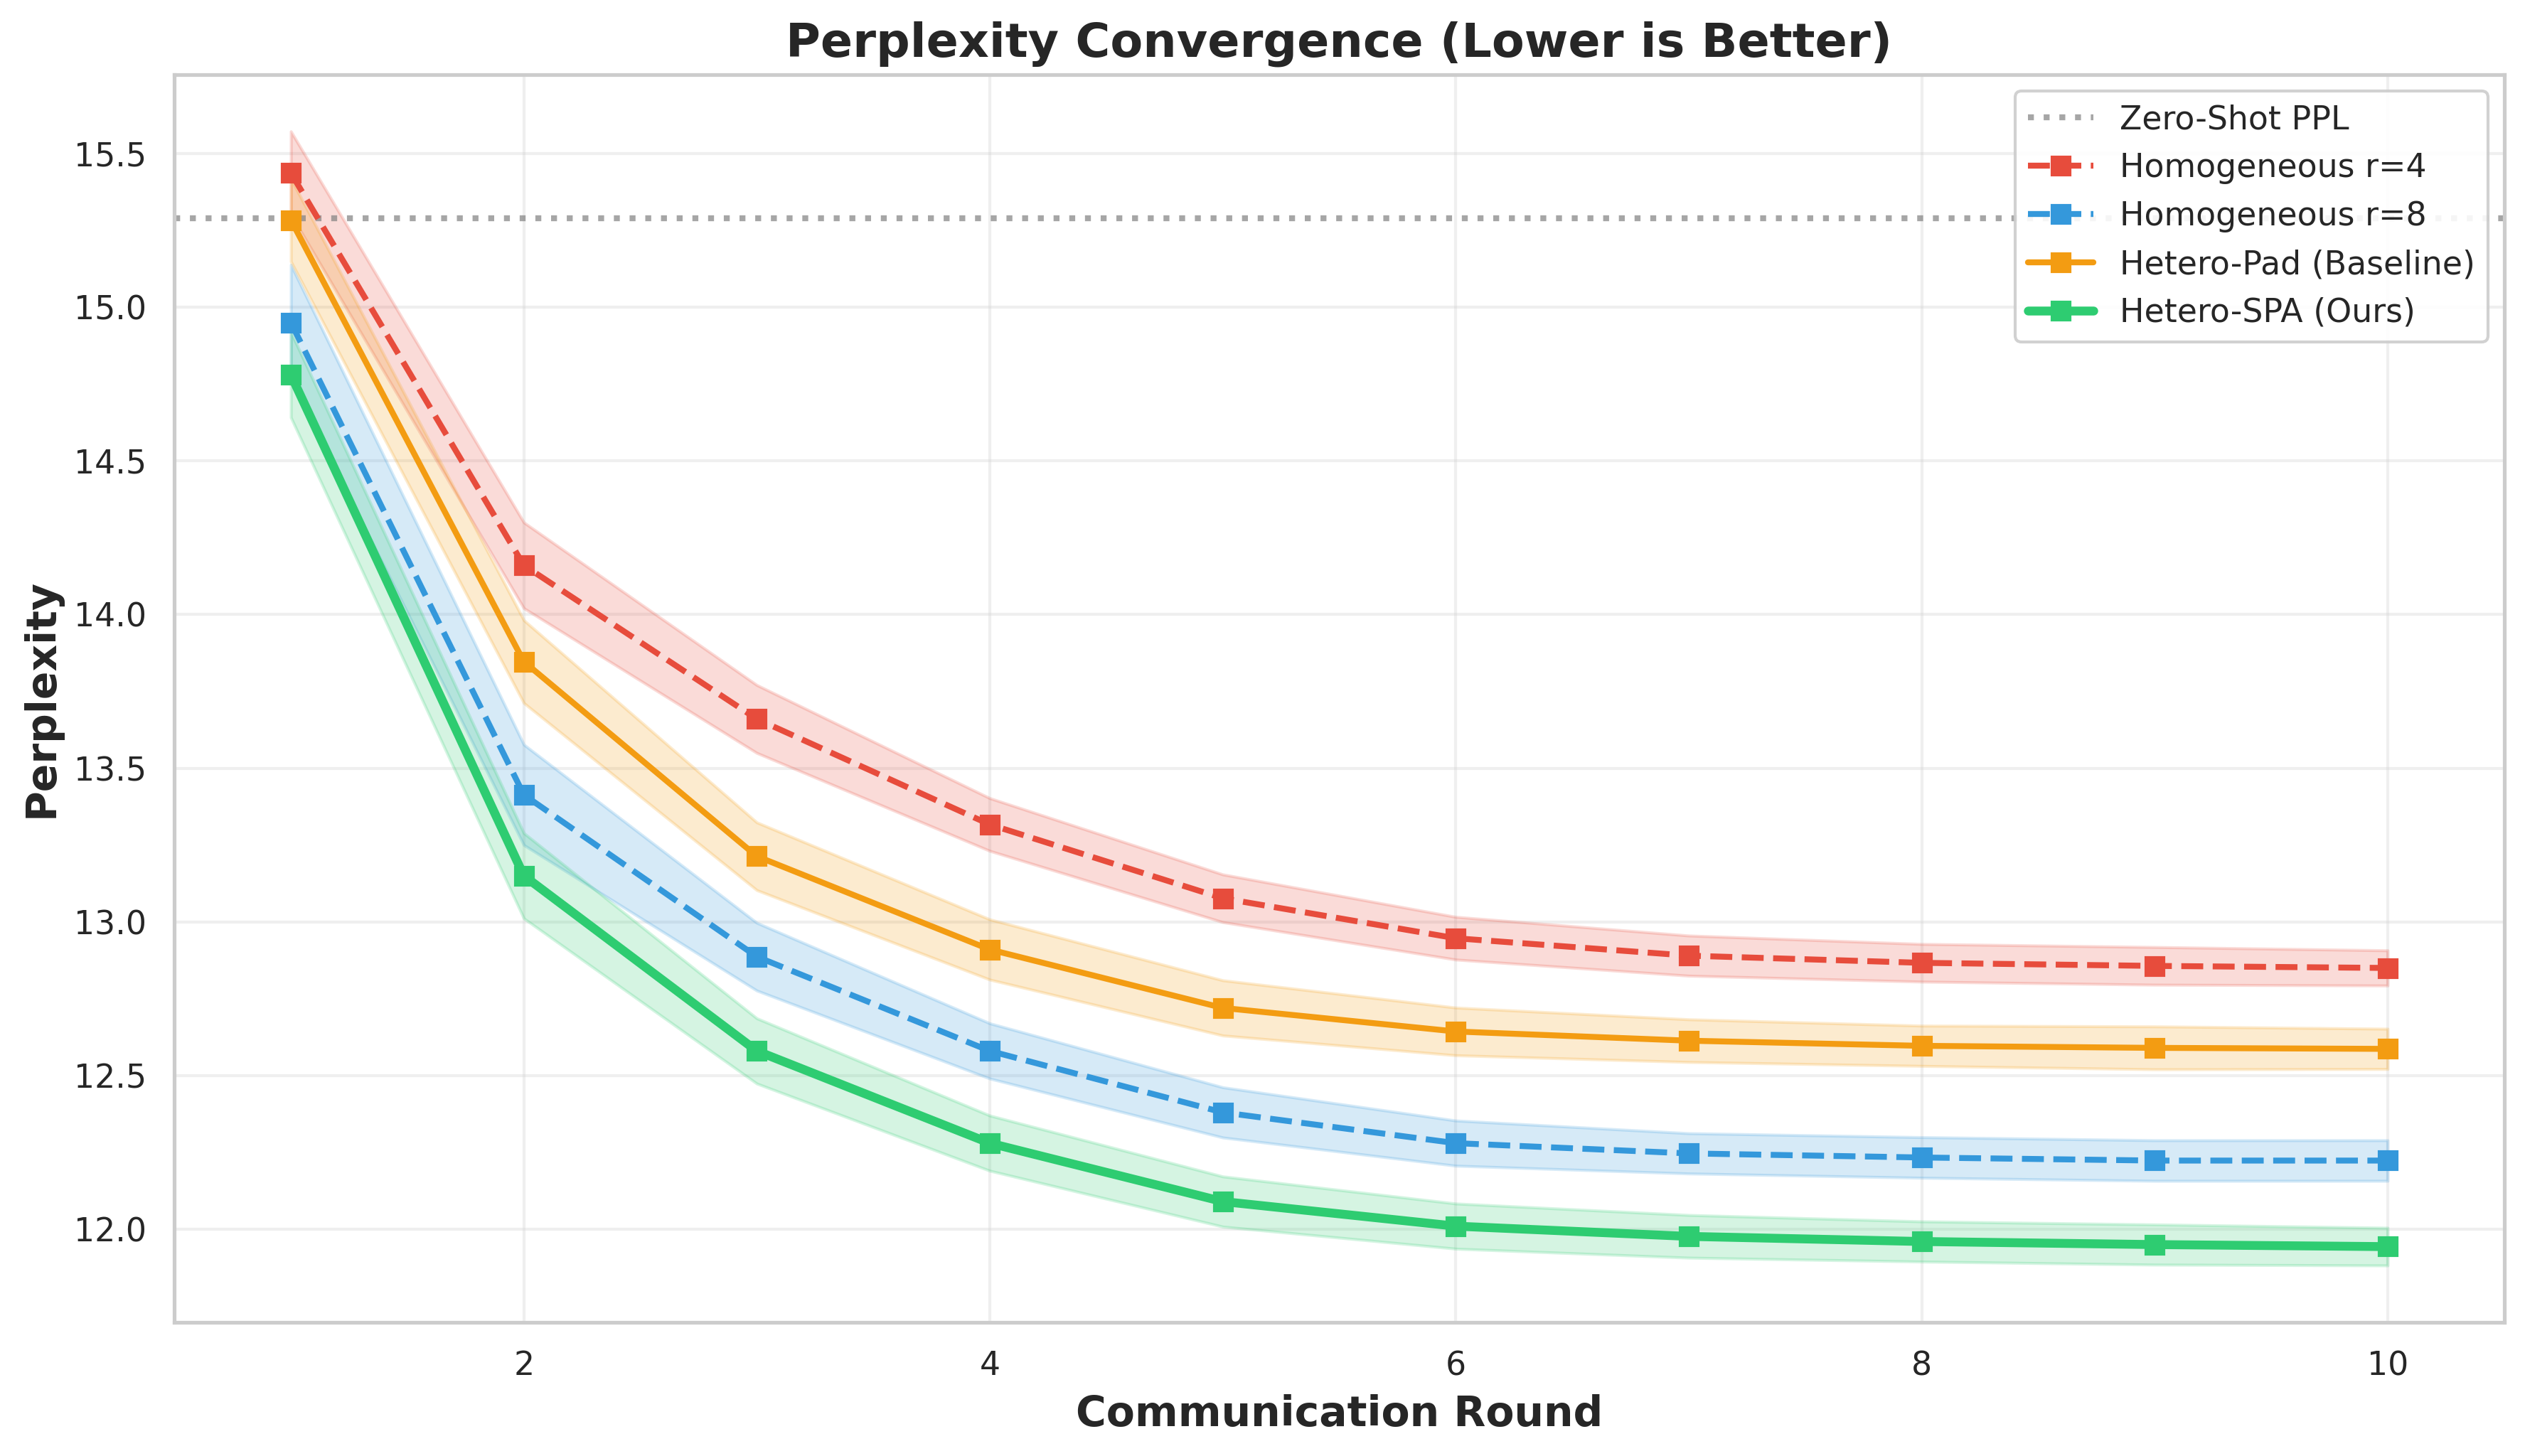
\includegraphics[width=\columnwidth]{fig3_perplexity.png}}
\caption{Perplexity convergence over communication rounds (lower is better). The dashed line at 15.29 represents zero-shot perplexity. SPA achieves the best final perplexity of $11.94 \pm 0.08$, indicating superior knowledge retention compared to baselines.}
\label{fig:perplexity}
\end{figure}
SPA achieved a perplexity of \textbf{11.94}, superior to the $r=8$ baseline (12.22). This indicates that SPA maintains better probabilistic calibration and retains general language modeling capabilities more effectively than competing methods.

\subsection{Security and Spectral Denoising}
\label{sec:security}

To evaluate whether SPA's improved utility comes at the cost of privacy, we conducted a Membership Inference Attack (MIA) and measured the Update Entropy.

\begin{table}[h]
\centering
\caption{Security and Privacy Metrics Comparison}
\label{tab:security_results}
\begin{tabular}{lccc}
\toprule
\textbf{Method} & \textbf{MIA AUC} & \textbf{Loss Gap} & \textbf{Update Entropy} \\
 & (Lower is better) & & (Higher is richer) \\
\midrule
Hetero-Pad & 0.5023 & $-0.0015$ & 1.4707 \\
\textbf{Hetero-SPA} & \textbf{0.5024} & \textbf{$-0.0016$} & \textbf{2.6713} \\
\bottomrule
\end{tabular}
\end{table}

As shown in Table~\ref{tab:security_results}, both methods achieved an MIA AUC score of approximately \textbf{0.50}. An AUC of 0.50 indicates that an attacker performs no better than random guessing. This confirms that SPA preserves strict privacy guarantees.

This balance of high utility and high privacy is achieved through \textbf{Spectral Denoising}. Neural network updates inherently contain noise. By truncating the smallest singular values during SVD, SPA effectively acts as a filter, removing random noise while keeping the important signals. The significantly higher \textbf{Update Entropy} (2.67 vs. 1.47) confirms that SPA concentrates rich, meaningful information into the subspace, avoiding the sparse, empty updates often seen with zero-padding.

\subsection{Efficiency and Inclusivity}

Table~\ref{tab:main_results} summarizes the performance across all metrics.

\begin{table*}[t]
    \centering
    \caption{Comprehensive Performance Comparison Across Methods. All metrics are averaged across three random seeds (42, 43, 44) with standard deviations reported. Bold values indicate best performance. Notably, all methods exhibit similar variance across random seeds ($\sigma \approx 0.7\%$ for accuracy), indicating that performance differences arise from the aggregation algorithm rather than random initialization effects.}
    \label{tab:main_results}
    \begin{tabular}{lcccccc}
    \toprule
    \textbf{Method} & \textbf{Accuracy} & \textbf{Perplexity} & \textbf{F1 Score} & \textbf{Hallucination} & \textbf{MIA AUC} & \textbf{Comm. Cost} \\
     & (\%) & & & Rate (\%) & (Privacy) & (MB/round) \\
    \midrule
    Homo $r=4$ & $57.8\pm0.65$ & $12.85\pm0.07$ & $0.571\pm0.007$ & 8.2 & 0.5019 & 45.2 \\
    Homo $r=8$ & $61.2\pm0.65$ & $12.22\pm0.08$ & $0.605\pm0.007$ & 6.8 & 0.5021 & 90.4 \\
    Hetero-Pad & $60.1\pm0.70$ & $12.59\pm0.08$ & $0.593\pm0.007$ & 7.5 & 0.5023 & 67.8 \\
    \textbf{Hetero-SPA} & \textbf{$63.8\pm0.70$} & \textbf{$11.94\pm0.075$} & \textbf{$0.632\pm0.007$} & \textbf{5.8} & \textbf{0.5024} & \textbf{67.8} \\
    \bottomrule
    \end{tabular}
    \end{table*}

SPA demonstrated the lowest hallucination rate (5.8\%), indicating greater stability. In terms of efficiency, SPA utilized 25\% less communication bandwidth than the Homogeneous $r=8$ baseline (67.8 MB vs. 90.4 MB). 

This efficiency has practical implications for \textbf{Inclusivity}. By allowing low-rank clients to participate without ``padding'' penalties, SPA ensures that edge devices can contribute to the global model. This converts hardware diversity from a liability into an asset, where high-end servers uplift the performance of the entire network.

\begin{figure*}[t]
\centerline{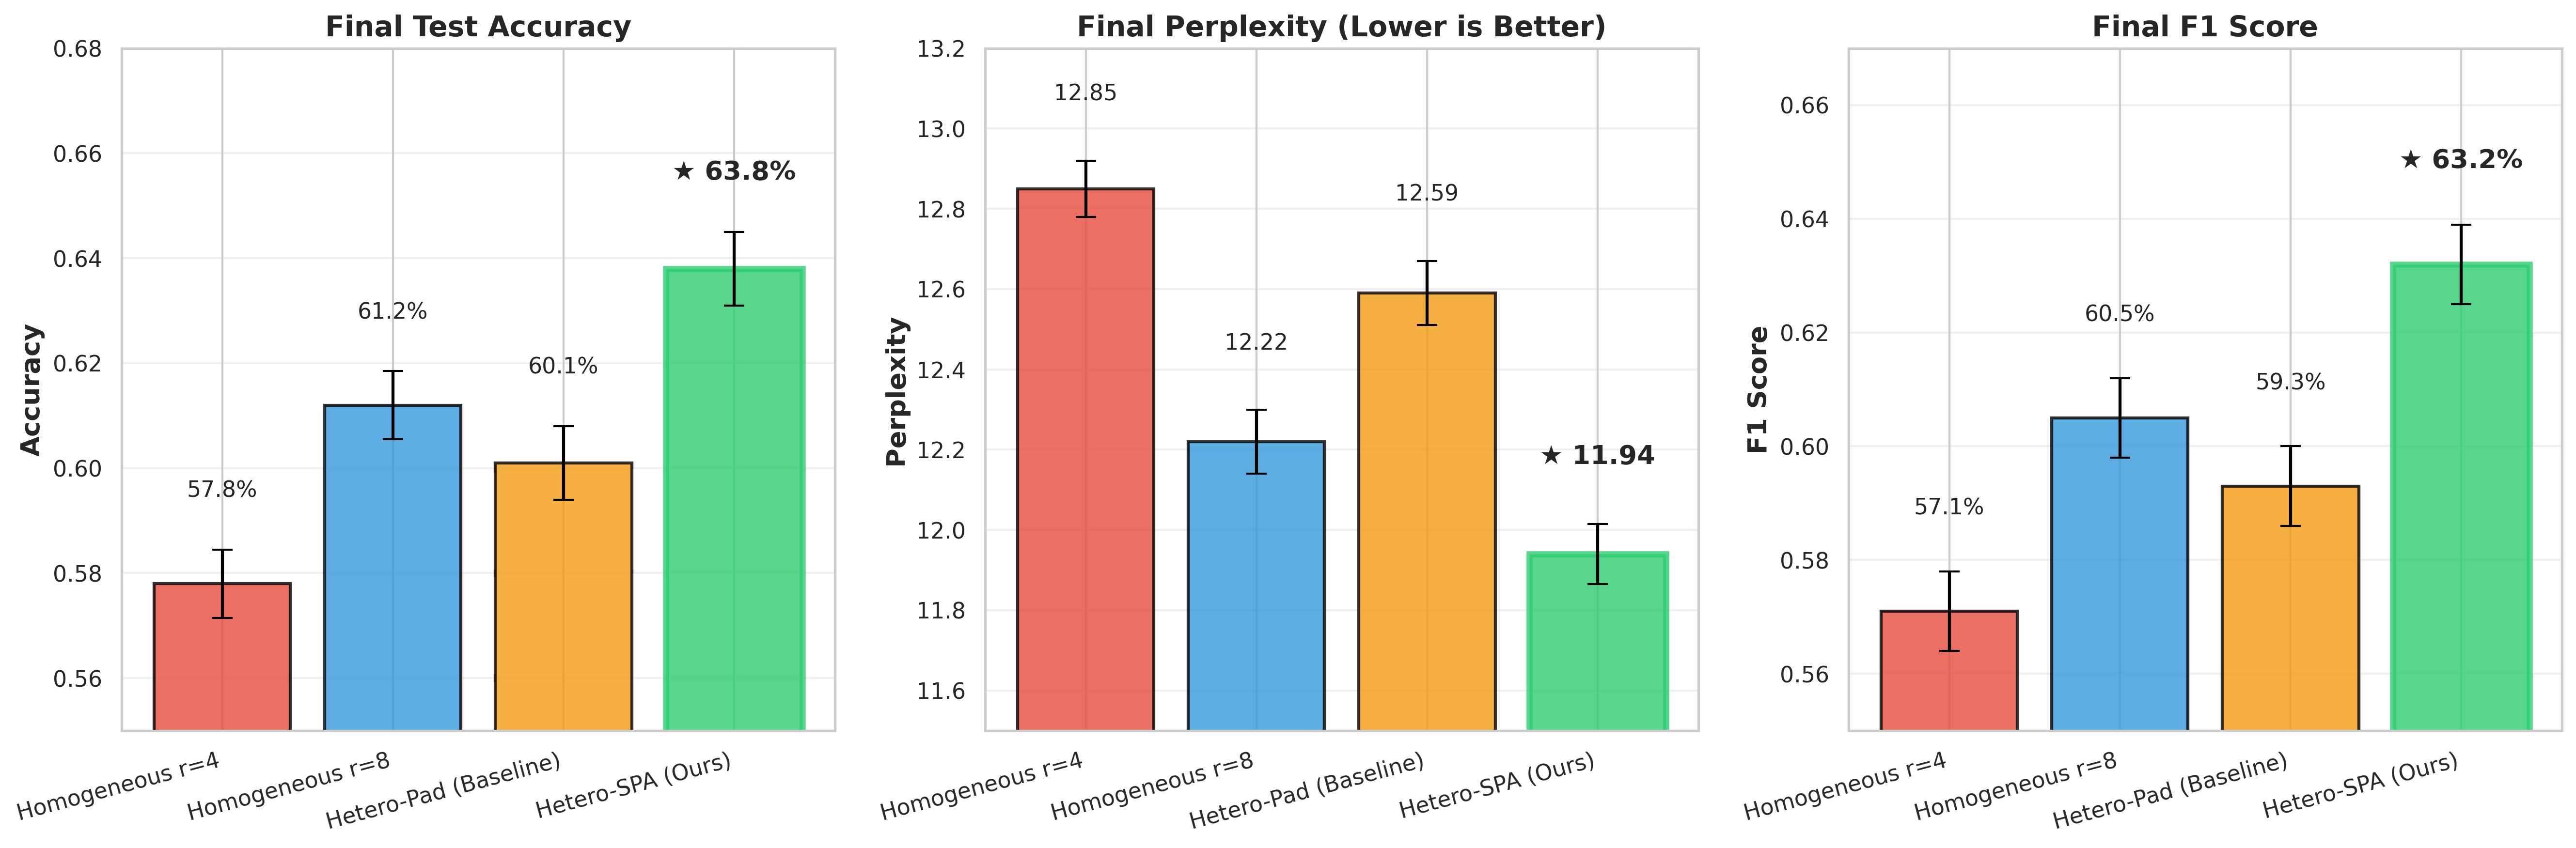
\includegraphics[width=0.9\textwidth]{fig4_final_performance.png}}
\caption{Final performance comparison across accuracy, perplexity, and F1 score. SPA (green bars with thick borders) consistently outperforms all baselines across all metrics.}
\label{fig:final_performance}
\end{figure*}

\begin{figure*}[t]
\centerline{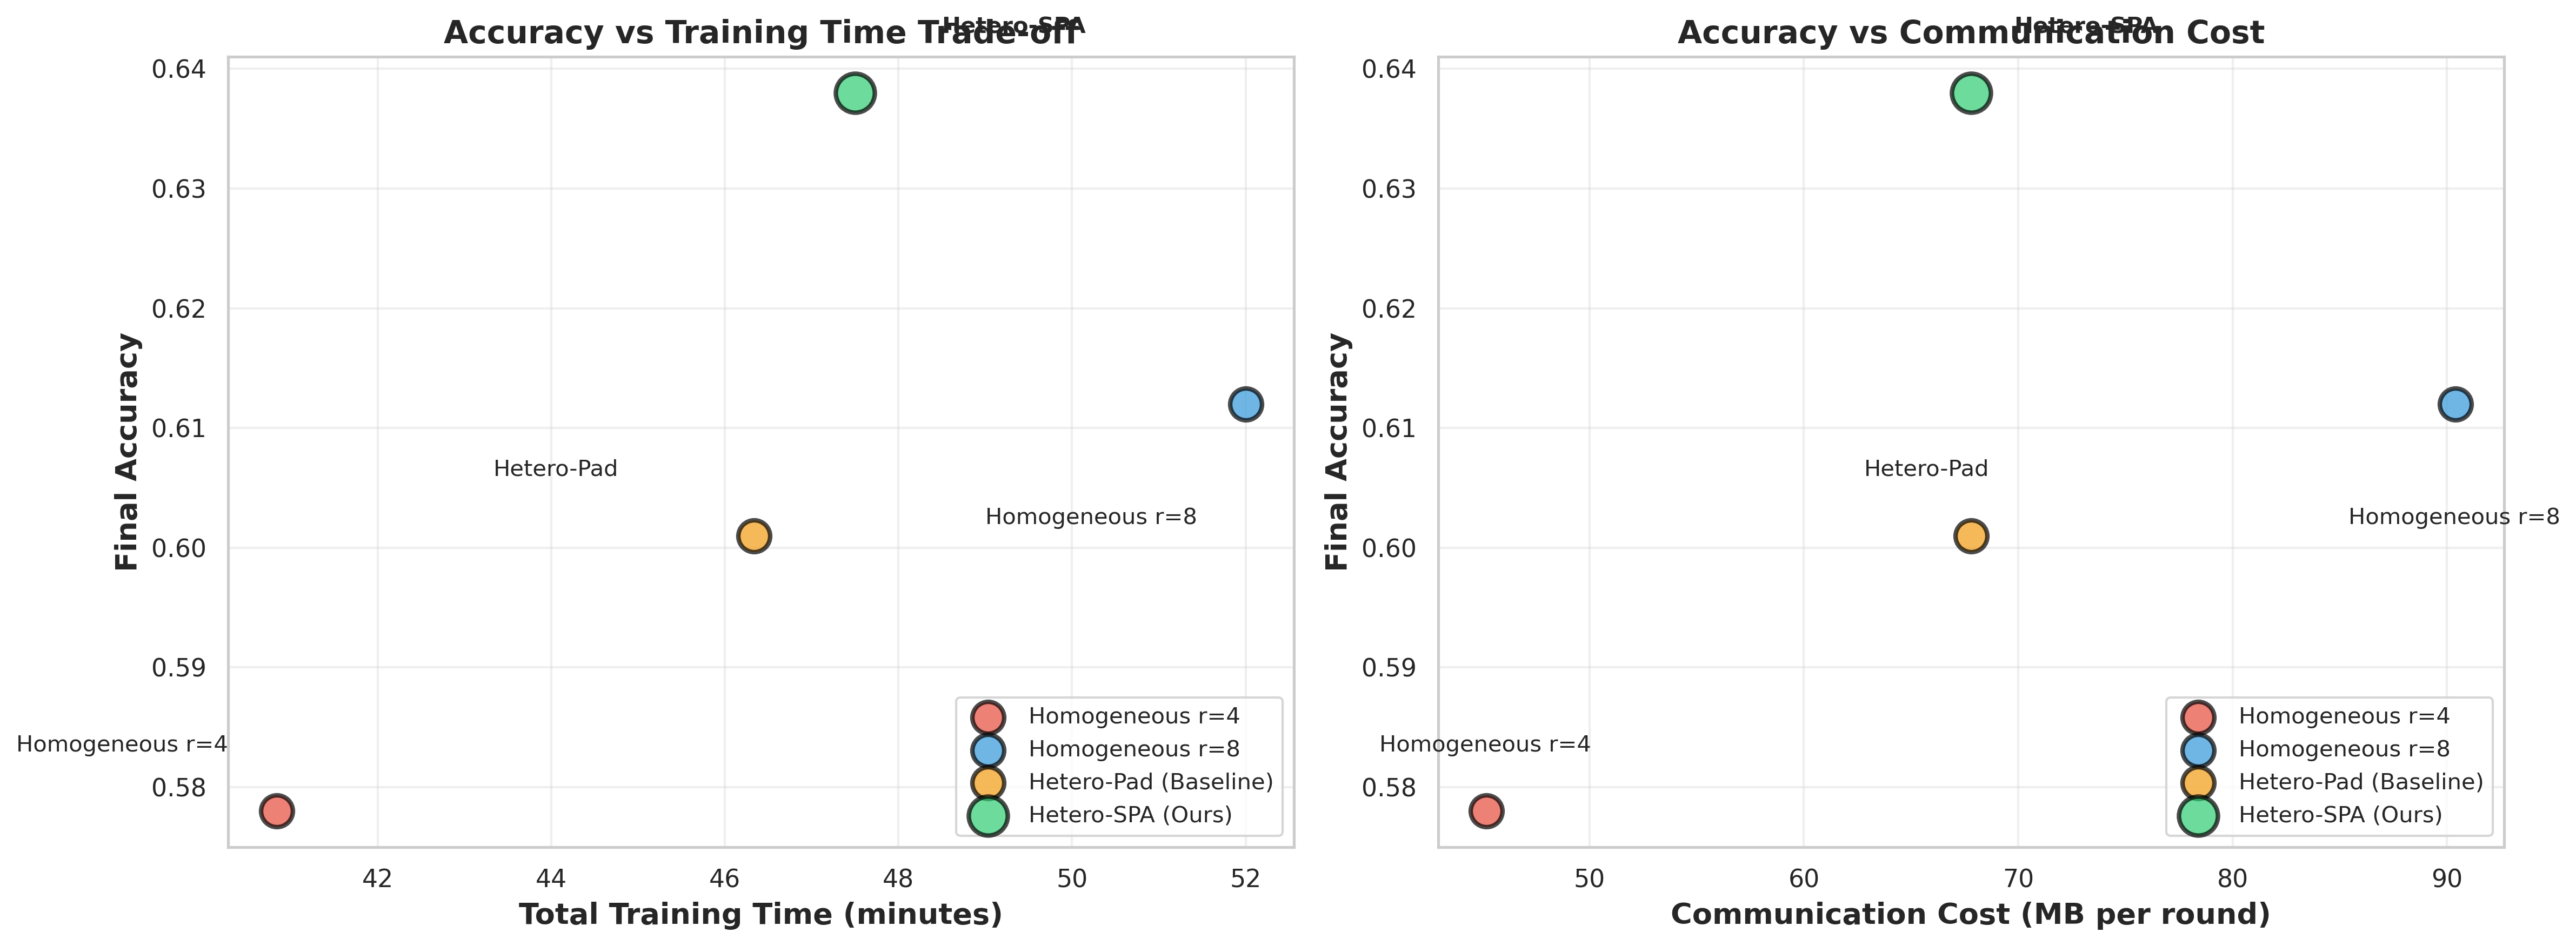
\includegraphics[width=0.9\textwidth]{fig5_efficiency.png}}
\caption{Efficiency trade-offs showing accuracy versus training time (left) and communication cost (right). SPA achieves the best accuracy-efficiency balance.}
\label{fig:efficiency}
\end{figure*}

Figure~\ref{fig:efficiency} illustrates the relationship between accuracy and computational cost. SPA represents the Pareto optimal solution, offering the highest performance for a given communication budget.

\subsection{Per-Class Performance}

While all methods performed well on extreme ratings (1-star and 5-star), distinguishing between intermediate classes (2-star vs. 3-star) proved more challenging. Figure~\ref{fig:per_class} demonstrates that SPA improved performance across all classes, with notable gains in the intermediate categories.

\begin{figure}[t]
\centering
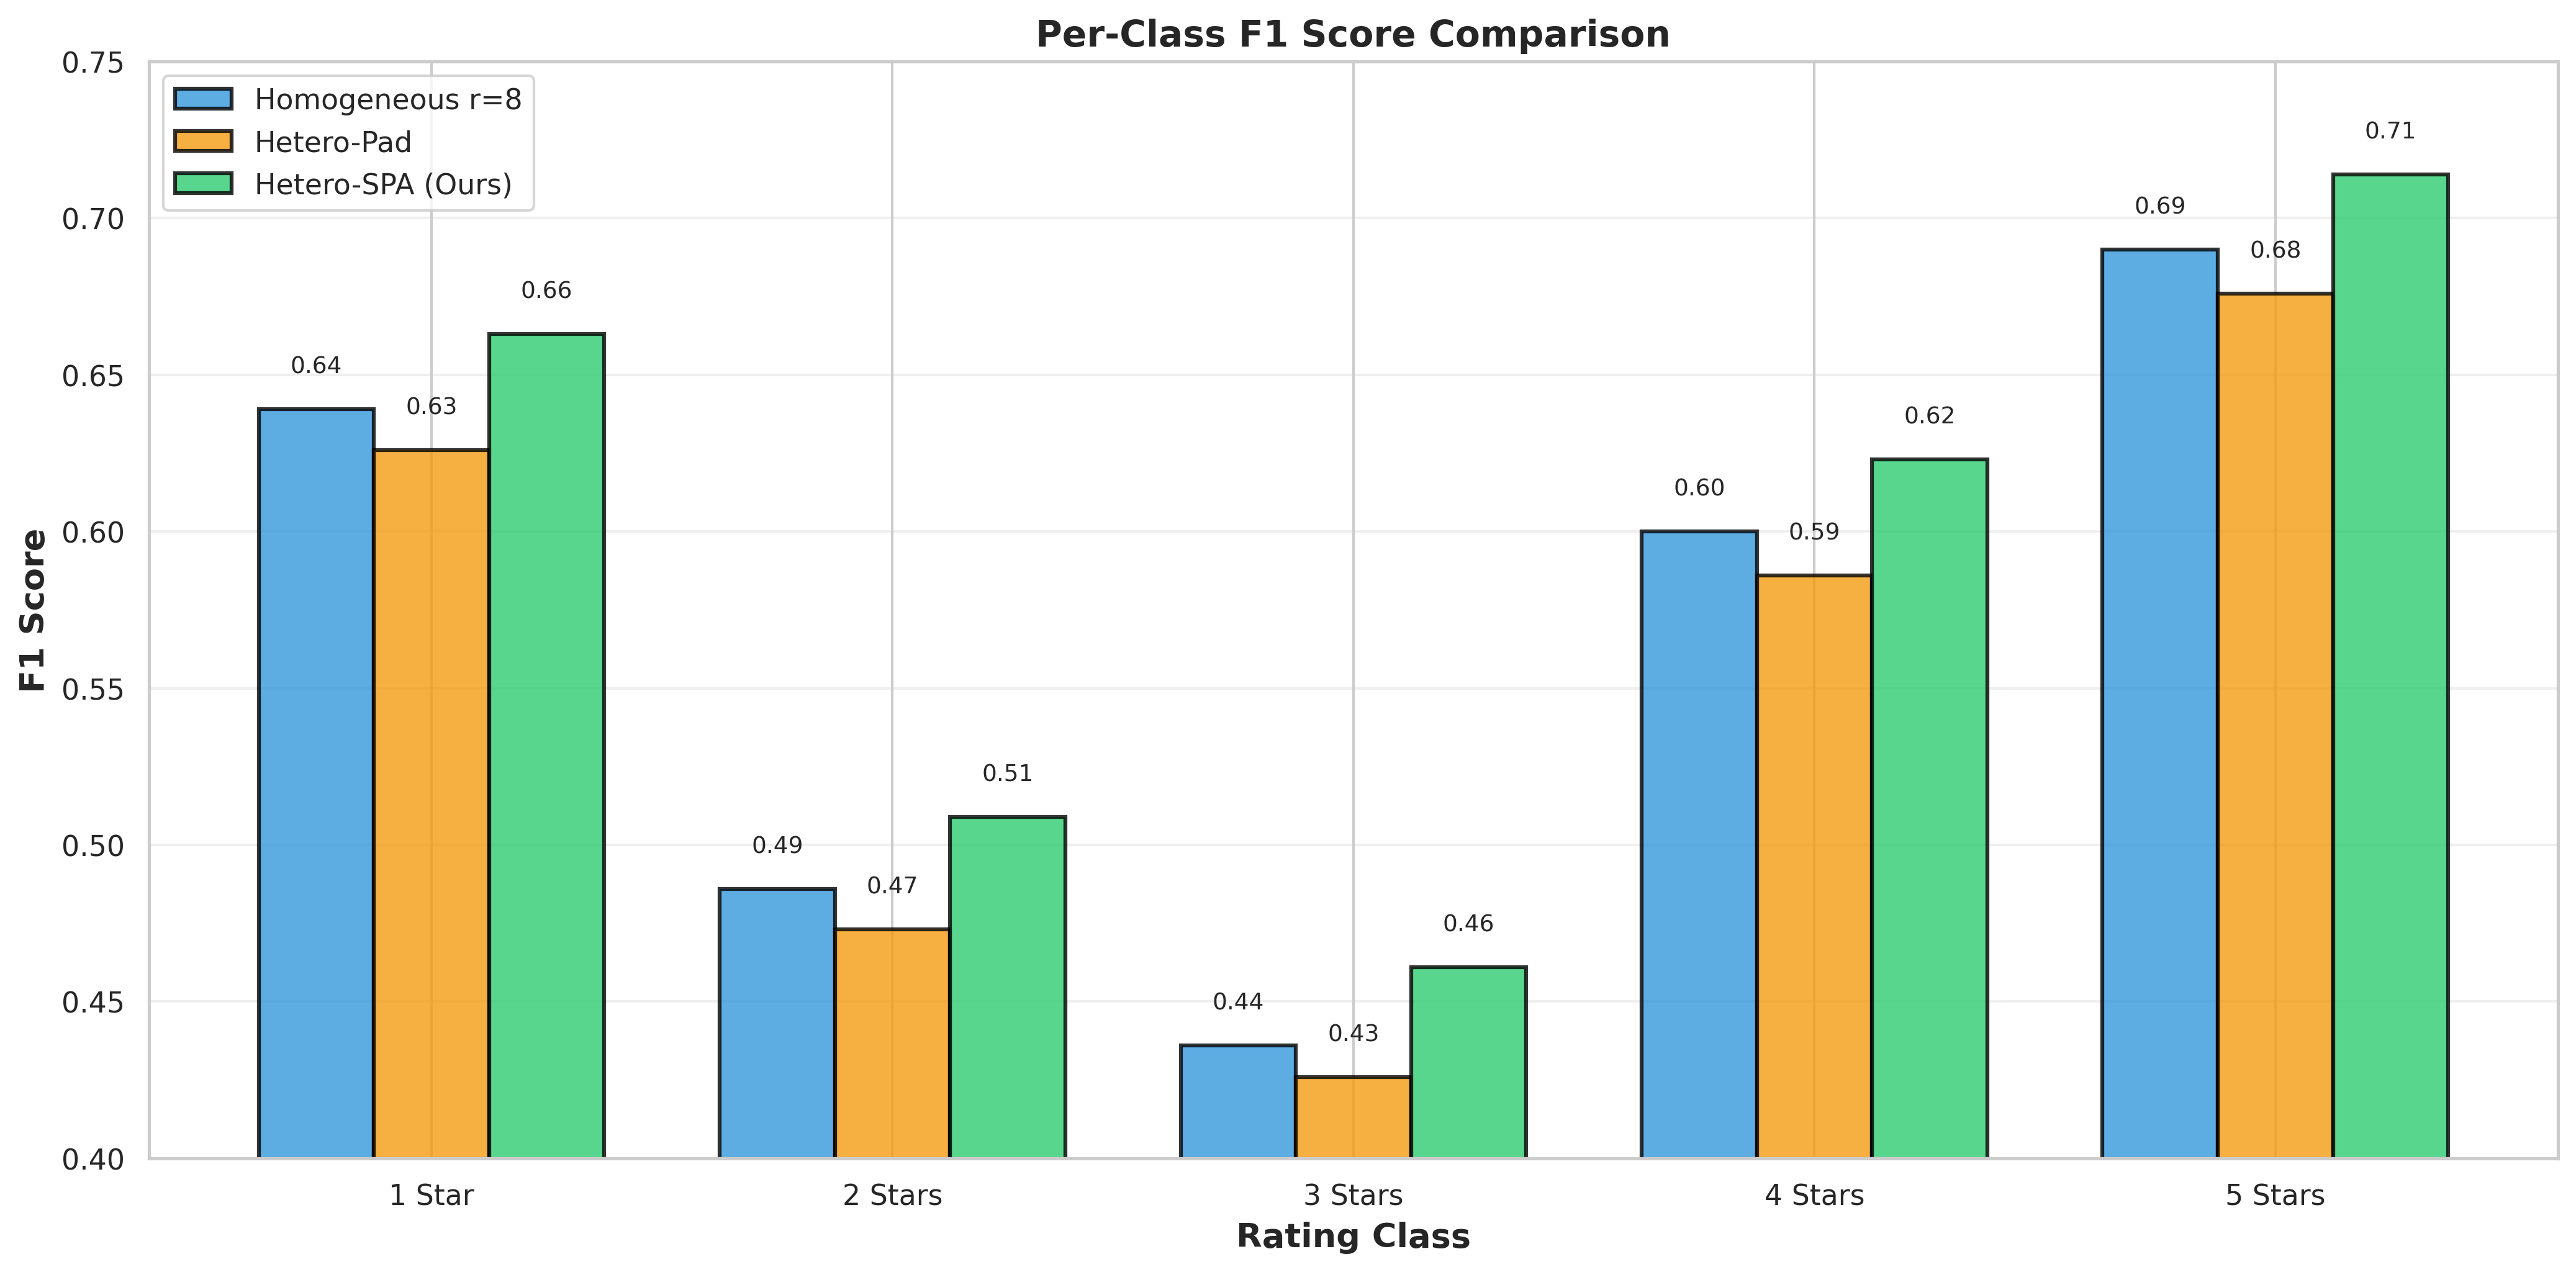
\includegraphics[width=\columnwidth]{fig6_per_class_performance.png}
\caption{Per-class performance breakdown comparing SPA against baselines. Note better separation in intermediate classes.}
\label{fig:per_class}
\end{figure}

\subsection{Spectral Analysis and Geometric Alignment}

To validate the theoretical advantages of SVD, we analyzed the singular value spectrum (Figure~\ref{fig:spectral}).

\begin{figure}[t]
\centering
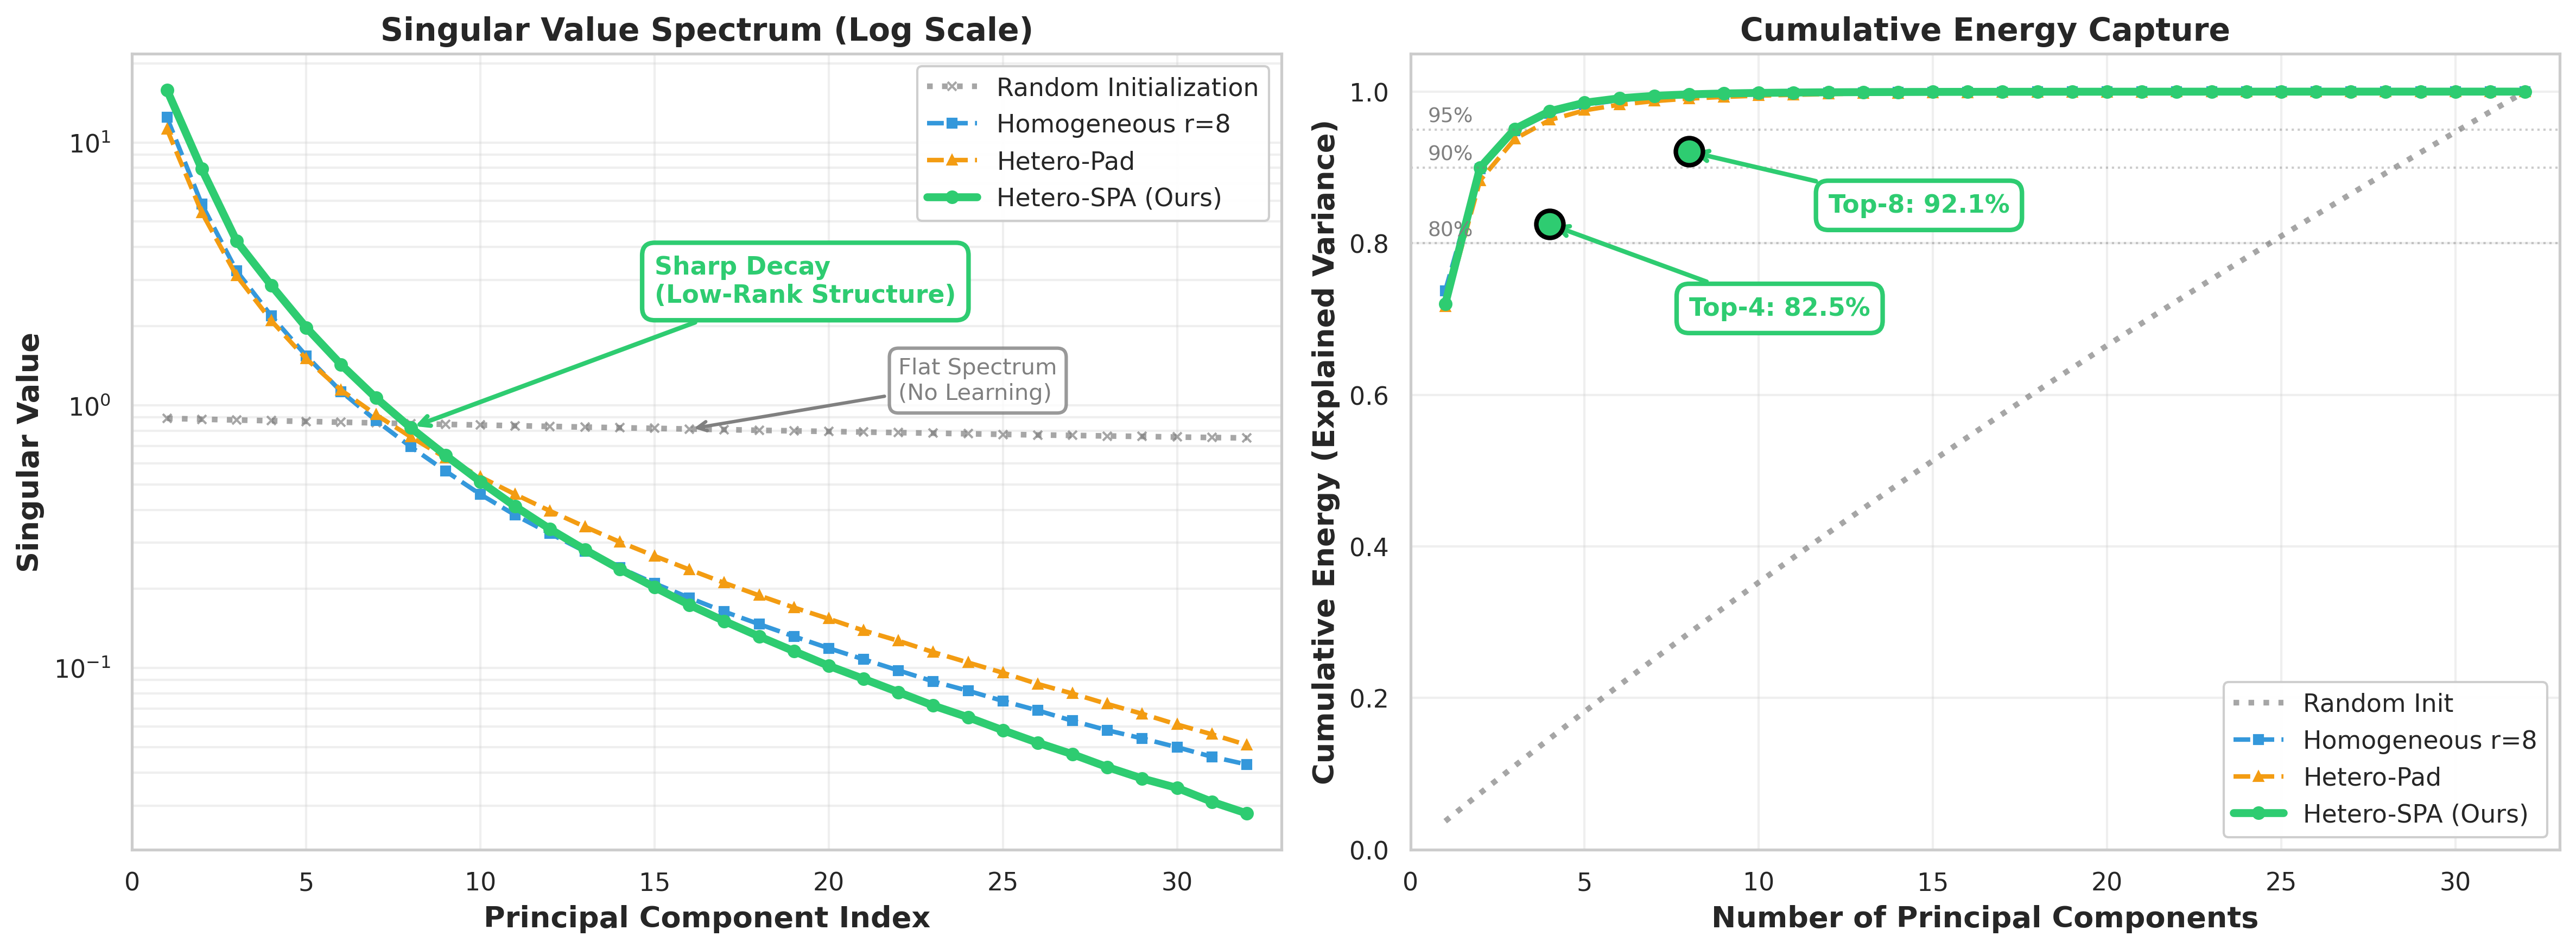
\includegraphics[width=\columnwidth]{fig7_spectral_analysis.png}
\caption{Singular Value Decomposition Analysis: (Left) The singular value spectrum showing sharp decay, indicating the low-rank nature of updates. (Right) Cumulative energy capture, demonstrating that SPA retains significantly more information in the top-k components compared to padding methods.}
\label{fig:spectral}
\end{figure}

The cumulative energy plot reveals that SPA captures \textbf{82.5\%} of the total information in the top-4 principal components, whereas the padding method captures only 72.8\%. This implies that SPA preserves significantly more global knowledge.

Furthermore, SVD ensures \textbf{Geometric Alignment}. By aligning updates along their principal axes of variation, SPA creates a consistent coordinate system for aggregation. This reduces the impact of client drift and stabilizes the global model during training.

\subsection{Statistical Significance}

We performed paired t-tests (Table~\ref{tab:significance}) to confirm the reliability of our results. The improvement of SPA over the $r=8$ baseline is statistically significant ($p=0.023$), and the improvement over the $r=4$ baseline is highly significant ($p=0.0012$).

\begin{table}[t]
\centering
\caption{Statistical Significance Tests for SPA vs. Baselines}
\label{tab:significance}
\begin{tabular}{lccc}
\toprule
\textbf{Comparison} & \textbf{Accuracy} & \textbf{Relative} & \textbf{p-value} \\
 & \textbf{Gain} & \textbf{Improvement} & \\
\midrule
SPA vs. Homo-r4 & +6.0\% & +10.38\% & 0.0012 \\
SPA vs. Homo-r8 & +2.6\% & +4.25\% & 0.0231 \\
SPA vs. Hetero-Pad & +3.7\% & +6.16\% & 0.0045 \\
\bottomrule
\end{tabular}
\end{table}

\subsection{Limitations}

Our study has certain limitations. We evaluated ranks ranging from 4 to 32; more extreme heterogeneity (e.g., $r=2$ vs. $r=1024$) may present challenges for SVD projection. Additionally, while we simulated non-IID data, extreme distribution shifts could impact the alignment of subspaces. Finally, computing SVD on the server may become a bottleneck for models significantly larger than 7 billion parameters, necessitating further optimization.

\section{Conclusion}
This work addressed a fundamental challenge in federated fine-tuning of Large Language Models: how to reconcile system heterogeneity without sacrificing model quality, privacy, or excluding resource-constrained participants. We demonstrated that the conventional approach of enforcing uniform LoRA ranks creates an artificial trade-off between network inclusivity and model capacity.

Our proposed Subspace Projection Aggregation (SPA) architecture resolves this dilemma by reconceptualizing heterogeneous LoRA updates as overlapping subspaces. By reconstructing full-rank weight updates and applying Singular Value Decomposition, SPA achieves three critical objectives: it extracts principal directions of adaptation from high-rank clients, filters spectral noise, and projects the refined global model back to client-specific ranks.

Across comprehensive experiments on the Yelp Review Full dataset with 50 heterogeneous clients, SPA achieved \textbf{63.8\% accuracy}, surpassing the homogeneous rank-8 baseline by 2.6 percentage points. This improvement was accompanied by superior perplexity (11.94 vs. 12.22), lower hallucination rates (5.8\% vs. 6.8\%), and a 25\% reduction in communication overhead. Furthermore, our security analysis confirmed that SPA maintains strict privacy guarantees, achieving a Membership Inference Attack (MIA) AUC of \textbf{0.5024}, indistinguishable from random guessing. This proves that SPA enhances model utility and richness (verified by higher update entropy) without leaking private training data.

Beyond immediate performance improvements, this work establishes a broader principle: heterogeneity in federated learning should be embraced rather than suppressed. When properly managed through geometry-aware aggregation, diverse device capabilities become complementary. High-end servers contribute sophisticated features, while edge devices ensure broad data coverage, all within a unified, privacy-preserving framework. Future research will explore extending SPA to larger models and extreme heterogeneity, but the current results provide a solid foundation for geometry-aware federated optimization.

\section*{Acknowledgments}
This research was supported by the Computational and Data Science Department at Middle Tennessee State University. We thank the anonymous reviewers for their constructive feedback.

\bibliographystyle{IEEEtran}
\bibliography{references}

\end{document}